% =====================================================================
% Generative AI -- Assignment 1: technical report (IEEE conference format)
%
% Compile with pdfLaTeX + BibTeX (Overleaf: upload the whole report/
% folder, main document = main.tex, compiler = pdfLaTeX).
%
% STATUS: DRAFT. No trained-model results exist yet. Every place that
% needs a result is marked twice:
%   - a LaTeX comment starting with  % TODO(results):
%   - a visible red marker produced by \TODO{...}
% Search for "TODO" before submission; report/README.md lists them all.
%
% Figures produced by the evaluation scripts are included automatically
% by \figOrTodo{path}{width}{description} as soon as the file exists in
% report/figures/; until then a red placeholder box is drawn instead.
% =====================================================================
\documentclass[conference]{IEEEtran}

\usepackage[T1]{fontenc}
\usepackage{cite}
\usepackage{amsmath,amssymb}
\usepackage{graphicx}
\usepackage{booktabs}
\usepackage{xcolor}
\usepackage{tikz}
\usetikzlibrary{positioning,arrows.meta,shapes,fit}
\usepackage{url}
\usepackage[hidelinks]{hyperref}

% ---------------------------------------------------------------------
% Helper macros
% ---------------------------------------------------------------------
% Visible placeholder for anything that is not finished yet.
\newcommand{\TODO}[1]{\textcolor{red}{[TODO: #1]}}
% File names and paths in typewriter font (underscores are safe; lines may
% break after "/", "_", "." and "-").
\DeclareUrlCommand\filepath{\urlstyle{tt}}
\def\UrlBreaks{\do\/\do\_\do\.\do\-}
\DeclareRobustCommand{\file}[1]{\expandafter\filepath\expandafter{\detokenize{#1}}}
% Include a figure if the file exists, otherwise draw a red placeholder.
%   #1 path relative to report/, #2 width, #3 what the figure must show
\newcommand{\figOrTodo}[3]{%
  \IfFileExists{#1}%
    {\includegraphics[width=#2]{#1}}%
    {\fbox{\parbox{0.92\linewidth}{\centering\footnotesize
      \TODO{#3}\\[2pt]\file{#1}}}}}
% Empty table cell waiting for a number.
\newcommand{\na}{--}

\emergencystretch=2em

\begin{document}

\title{Restoring Corrupted Images and Generating Facial Sketches:\\
Autoencoders, Hard and Soft Expert Routing, and a Style-Conditioned GAN}

\author{\IEEEauthorblockN{TODO: Student Name}
\IEEEauthorblockA{TODO: Roll number, Department, University\\
TODO: email}}

\maketitle

% =====================================================================
\begin{abstract}
We design, train, evaluate and deploy four related generative image
systems. Three of them restore $128\times128$ images of the Oxford-IIIT
Pet dataset that are corrupted at runtime by salt-and-pepper noise,
Gaussian blur or rectangular occlusion: (1)~a single universal denoising
autoencoder with a compressed spatial bottleneck, (2)~a corruption
classifier that hard-routes each input to one of three specialist
autoencoders or to an identity bypass, and (3)~a soft mixture-of-experts
in which a gate initialised from the classifier weights all four branches
and is fine-tuned jointly with the experts. The fourth system is a
style-conditioned conditional GAN with a U-Net generator and a PatchGAN
discriminator that translates FS2K face photographs into sketches in one of
three styles. Every model is tuned with Optuna, tracked in Weights \&
Biases, exported to ONNX and served by a FastAPI backend to a React
application that runs in Docker containers.
% TODO(results): one or two sentences with the headline test numbers of each task.
\TODO{Headline results: test PSNR/SSIM of Tasks 1--3 on corrupted inputs,
classifier macro-F1, oracle vs.\ predicted routing gap, Task~4 test SSIM;
fill in from \file{report/results/*.csv} once evaluation has run.}
\end{abstract}

\begin{IEEEkeywords}
denoising autoencoder, image restoration, mixture of experts,
conditional GAN, hyperparameter optimisation, ONNX deployment
\end{IEEEkeywords}

% =====================================================================
\section{Introduction}
\label{sec:intro}

Images met in practice are often degraded, and the type of degradation is
usually not known in advance. This assignment studies how far one learned
model can restore several corruption types without being told which one is
present, and whether making the corruption type explicit---first through a
hard decision and then through a learned soft weighting---changes that
picture. A fourth task turns from restoration to paired generation: a
conditional GAN that draws a sketch of a face photograph in a chosen style.

The four systems are:
\begin{enumerate}
  \item \emph{Universal Restoration} (Task~1): one convolutional denoising
  autoencoder for clean, noisy, blurred and occluded inputs
  (Section~\ref{sec:task1}).
  \item \emph{Hard-Routed Restoration} (Task~2): a four-class corruption
  classifier that selects one of three specialist autoencoders, or returns
  a clean input unchanged (Section~\ref{sec:task2}).
  \item \emph{Soft Mixture-of-Experts Restoration} (Task~3): a gate that
  assigns a continuous weight to the identity branch and the three experts,
  trained jointly with them (Section~\ref{sec:task3}).
  \item \emph{Face-to-Sketch Generator} (Task~4): a U-Net generator and a
  PatchGAN discriminator, both conditioned on a learned style embedding
  (Section~\ref{sec:task4}).
\end{enumerate}

All models are tuned with Optuna, logged in Weights \& Biases (W\&B),
exported to ONNX, and served through a single browser application
(Section~\ref{sec:app}). Our emphasis throughout is on making each
requirement \emph{checkable}: the data split and every validation and test
corruption are stored in committed files, the routing decisions and the
gate's behaviour are evaluated against stated numerical criteria, and every
exported model is compared numerically with its PyTorch counterpart.
Design alternatives and the reasons for each choice are given with the
corresponding method; the experimental setup is described in
Section~\ref{sec:setup}, limitations in Section~\ref{sec:limitations}.

% =====================================================================
\section{Related Work}
\label{sec:related}

\subsection{Denoising autoencoders and restoration losses}
Vincent \emph{et al.}~\cite{vincent2008extracting} train autoencoders to
reconstruct a clean input from a deliberately corrupted copy, so that the
learned representation must capture structure rather than copy the input.
Tasks~1 and~2 apply the same principle with three corruption types and a
convolutional architecture. Ronneberger \emph{et
al.}~\cite{ronneberger2015unet} showed that skip connections between a
contracting and an expanding path preserve fine spatial detail; for an
autoencoder this is a double-edged property, because unrestricted skips
let the input bypass the bottleneck. For the decoder, Odena \emph{et
al.}~\cite{odena2016deconvolution} explain how transposed convolutions with
uneven kernel overlap produce checkerboard artefacts and propose resizing
followed by a convolution instead. As a training and evaluation measure
next to the pixel-wise L1 error we use the structural similarity index
(SSIM) of Wang \emph{et al.}~\cite{wang2004ssim}, which compares local
luminance, contrast and structure.

\subsection{Mixtures of experts}
Jacobs \emph{et al.}~\cite{jacobs1991adaptive} introduced adaptive
mixtures of local experts, in which a gating network decides how much each
expert network contributes for a given input and the experts specialise on
different parts of the input space. Shazeer \emph{et
al.}~\cite{shazeer2017outrageously} scaled the idea with a sparsely gated
layer that activates only a few experts per example and added auxiliary
losses that discourage the gate from favouring a small subset of experts.
Our Task~3 model is a small, dense instance: four branches, all evaluated
for every image, with a squared-deviation balance term on the mean routing
weights.

\subsection{Conditional GANs for paired image translation}
Generative adversarial networks~\cite{goodfellow2014generative} train a
generator against a discriminator that separates real from generated
samples. Conditional GANs~\cite{mirza2014conditional} feed side information
to both networks. Isola \emph{et al.}~(pix2pix)~\cite{isola2017image}
combine a conditional adversarial loss with an L1 reconstruction term for
paired image-to-image translation, using a U-Net generator and a PatchGAN
discriminator that judges local patches. Task~4 follows this design and
adds a learned style condition. Heusel \emph{et
al.}~\cite{heusel2017gans} proposed the Fr\'echet Inception Distance (FID)
for comparing generated and real image sets; we discuss in
Section~\ref{sec:task4} why we did not select models by FID.

\subsection{Hyperparameter search and optimisation}
Optuna~\cite{akiba2019optuna} provides define-by-run search spaces, the
Tree-structured Parzen Estimator (TPE) sampler and pruning of unpromising
trials, all of which we use. For the classifier we use AdamW, which
decouples weight decay from the adaptive gradient
step~\cite{loshchilov2019decoupled}.

% =====================================================================
\section{Datasets and Corruption Protocol}
\label{sec:data}

\subsection{Oxford-IIIT Pet: preparation and split}
Tasks~1--3 use the Oxford-IIIT Pet dataset~\cite{parkhi2012cats}, which
contains photographs of 37 cat and dog breeds. The breed labels are not
used; the original images are the clean restoration targets. Every image
is converted to RGB and resized \emph{directly} to $128\times128$ with
bicubic interpolation. We considered resizing the short side and
centre-cropping, which preserves the aspect ratio, but rejected it because
it discards the image borders, and the application must apply the same
preprocessing to arbitrary uploads; a direct resize keeps the whole image at
the cost of distorting the aspect ratio of non-square photographs. To
avoid decoding JPEG files in every epoch and every Optuna trial, the
resized \emph{clean} images are cached once as one array per split
(\file{data/pet_128/}); no corrupted image is ever stored.

The official \texttt{trainval} list is sorted, shuffled with a NumPy
generator seeded with 42, and divided 80/20 into training and validation
sets; the official test list is kept aside until final evaluation. Instead
of recomputing the split from the seed in every script, the name lists are
saved once to \file{manifests/pet_split.json}, which every task reads, and
the preparation script raises an error if a recomputed split ever differs
from the saved file. Table~\ref{tab:pet_split} lists the resulting sizes.

\begin{table}[t]
\centering
\caption{Oxford-IIIT Pet split (seed 42) and corruption manifests.}
\label{tab:pet_split}
\footnotesize
\begin{tabular}{lrl}
\toprule
Set & Items & Content \\
\midrule
Training   & 2,944  & clean images; corrupted at runtime \\
Validation & 736    & clean images \\
Test       & 3,669  & official test list, held out \\
\midrule
Validation manifest & 2,944  & 736 images $\times$ 4 conditions \\
Test manifest       & 36,690 & 3,669 images $\times$ 10 conditions \\
\bottomrule
\end{tabular}
\end{table}

\subsection{Runtime corruption}
For every training image the data loader draws one of four input
conditions with equal probability---clean, salt-and-pepper noise, Gaussian
blur or rectangular occlusion---samples its severity, and applies it on the
fly, so each epoch sees new corruptions. The condition label is returned
with the image; Task~1 ignores it, Tasks~2 and~3 use it as the classification
target. Table~\ref{tab:corruptions} gives the complete configuration.

Each corruption is implemented as a \emph{sampler}, which returns plain
parameters (probability, kernel size and $\sigma$, rectangle coordinates),
and an \emph{apply} function, which takes them. This separation lets the
same code produce random training corruptions, replay stored validation and
test corruptions exactly, and be reimplemented for the application.
Salt-and-pepper noise acts on whole pixels: a selected pixel has all three
channels set to white or to black with equal probability; changing channels
independently would produce coloured specks rather than the black and white
pixels the specification describes. Blur uses torchvision's Gaussian blur
followed by clamping to $[0,1]$, which removes values slightly above 1
caused by floating-point rounding (found when the pipeline was first run on
the real data).

For occlusion, the requirement that one to three black rectangles
\emph{jointly} cover 10--35\% of the image raises the question of overlaps.
Rejecting overlapping samples on their union area is valid but rejects many
samples at high coverage. We instead split the target area between the
rectangles with random shares, give each a random aspect ratio, and place
them so that they do not overlap; the union area then equals the sum of the
areas, and a sample is accepted when its measured coverage lies in the
training range (or within 0.01 of a fixed test target). Over 2,000 draws the
sampler needed on average 1.0 attempts at the low and medium test
severities, 1.104 at the high severity (maximum 4) and 1.0185 with the
training ranges (maximum 2).

\begin{table*}[t]
\centering
\caption{Complete corruption configuration. Training severities are sampled
anew for every loaded image; the test severities are fixed. Validation
severities are drawn from the training ranges with a stored per-entry seed.}
\label{tab:corruptions}
\footnotesize
\begin{tabular}{@{}lp{6.0cm}ccc@{}}
\toprule
Condition & Training configuration & Test: low & Test: medium & Test: high \\
\midrule
Clean & image unchanged & \multicolumn{3}{c}{unchanged (one entry per test image)} \\
Salt-and-pepper & pixel probability $p\sim U(0.02,0.15)$; black/white with prob.\ 0.5
  & $p=0.03$ & $p=0.08$ & $p=0.15$ \\
Gaussian blur & kernel $k\in\{3,5,7\}$, $\sigma\sim U(0.5,2.5)$
  & $(k,\sigma)=(3,0.7)$ & $(5,1.5)$ & $(7,2.5)$ \\
Occlusion & 1--3 black, non-overlapping rectangles; union coverage $\in[0.10,0.35]$
  & 1 rect., $\approx$10\% & 2 rect., $\approx$20\% & 3 rect., $\approx$35\% \\
\midrule
\multicolumn{5}{@{}p{0.9\textwidth}@{}}{\emph{Occlusion sampler:} area shares
  $U(0.5,1.5)$, aspect ratio (h/w) $U(0.5,2.0)$, test tolerance $\pm0.01$, up to 50
  placement tries per rectangle and 1,000 attempts per sample.
  \emph{Measured test coverage:} low 0.0976--0.1025, medium 0.1956--0.2042,
  high 0.3439--0.3566.} \\
\bottomrule
\end{tabular}
\end{table*}

\subsection{Deterministic validation and test manifests}
Validation and test corruptions must be deterministic. Both manifests are
generated once, stored as JSON Lines in \file{manifests/} and committed.
Each entry records the image index, the condition, its severity, the
parameters (probability, kernel size and $\sigma$, or the rectangle
coordinates) and a random seed; for salt-and-pepper the seed fixes which
pixels are changed. The test manifest has ten entries per test image: the
clean image and each corruption at the three fixed severities. For the
validation manifest we compared one random condition per image (736 items,
about 184 per condition, balanced only approximately) with all four
conditions per image (2,944 items, exactly balanced); we chose the latter,
which makes the Optuna objective less noisy at negligible cost. Validation
severities are drawn from the \emph{training} ranges rather than the test
settings, so that hyperparameters are not tuned on the exact test
configuration. Unit tests confirm that two builds of each manifest are
identical and that a manifest item yields a bit-identical corrupted image
on repeated loads. Fig.~\ref{fig:corruption_preview} shows examples.

\begin{figure}[t]
\centering
\figOrTodo{figures/corruption_preview.png}{\columnwidth}{Corruption preview grid}
\caption{Examples of the test-manifest corruptions at the three fixed
severities (generated by \file{src/evaluation/preview_corruptions.py}).}
\label{fig:corruption_preview}
\end{figure}

\subsection{FS2K: split and paired augmentation}
Task~4 uses FS2K~\cite{fan2022facial}, which contains 2,104 paired face
photographs and sketches in three sketch styles. We use the official
\file{anno_train.json} and \file{anno_test.json} definitions (1,058 and
1,046 pairs according to the dataset repository). From the official
training portion, 15\% of the records of \emph{each style}
($\mathrm{round}(0.15\,n_{\mathrm{style}})$, seed 42) are held out for
validation, and the split is saved to \file{manifests/fs2k_split.json}.
An unstratified split was rejected because it could leave one style with
very few validation images. Each photograph is mapped to its sketch by the
naming rule of the dataset's own tooling, and both are converted to RGB and
resized directly to $128\times128$ (bicubic). Sketches are currently stored
with three channels.
% TODO(results): confirm sketch channel count from the prepare_fs2k output.
\TODO{Confirm from the output of \file{python -m src.data.prepare_fs2k}
how many sketches are greyscale and whether one output channel would
suffice; report original image sizes.}

Training augmentation follows pix2pix~\cite{isola2017image}: a random
horizontal flip, a resize to $143\times143$ and a random $128\times128$
crop. Independent augmentation of photo and sketch would destroy their
pixel correspondence, so both images are stacked into one tensor and
transformed with a single draw of the random parameters; a unit test checks
that a pair whose sketch is an exact copy of the photo remains identical
over 50 augmentations. Table~\ref{tab:fs2k_split} will list the per-style
counts.

\begin{table}[t]
\centering
\caption{FS2K split per sketch style.}
\label{tab:fs2k_split}
\footnotesize
\begin{tabular}{lrrr}
\toprule
Style & Train & Validation & Test \\
\midrule
Style 1 & \na & \na & \na \\
Style 2 & \na & \na & \na \\
Style 3 & \na & \na & \na \\
\midrule
Total   & \na & \na & \na \\
\bottomrule
\end{tabular}
\\[3pt]
% TODO(results): fill per-style counts from manifests/fs2k_split.json.
\TODO{Fill from \file{manifests/fs2k_split.json}.}
\end{table}

% =====================================================================
\section{Task 1: Universal Denoising Autoencoder}
\label{sec:task1}

\subsection{Architecture}
The model (Fig.~\ref{fig:task1_arch}) is a convolutional autoencoder
$\hat{x}=D(E(\tilde{x}))$, where $\tilde{x}$ is the corrupted input. A stem
convolution is followed by four stages that halve the resolution
($128\to64\to32\to16\to8$) with channels $c, c, 2c, 4c, 8c$ ($c$ is the
base width); each stage is a stride-2 $3\times3$ convolution and a second
$3\times3$ convolution, both with batch normalisation and ReLU. A $1\times1$
convolution maps the $8\times8\times8c$ feature to the bottleneck
$z\in\mathbb{R}^{C_z\times8\times8}$, where channel dropout
(\texttt{Dropout2d}) is applied during training. The decoder mirrors the
encoder with four stages of nearest-neighbour upsampling followed by two
$3\times3$ convolutions, and a final $3\times3$ convolution with a sigmoid
produces the image in $[0,1]$.

\begin{figure}[t]
\centering
% Task 1: universal denoising autoencoder (src/models/autoencoder.py).
% c = base_channels, C_z = latent_channels (both tuned by Optuna).
% Included from main.tex with % Task 1: universal denoising autoencoder (src/models/autoencoder.py).
% c = base_channels, C_z = latent_channels (both tuned by Optuna).
% Included from main.tex with % Task 1: universal denoising autoencoder (src/models/autoencoder.py).
% c = base_channels, C_z = latent_channels (both tuned by Optuna).
% Included from main.tex with \input{figures/tikz/task1_udae}.
\resizebox{\columnwidth}{!}{%
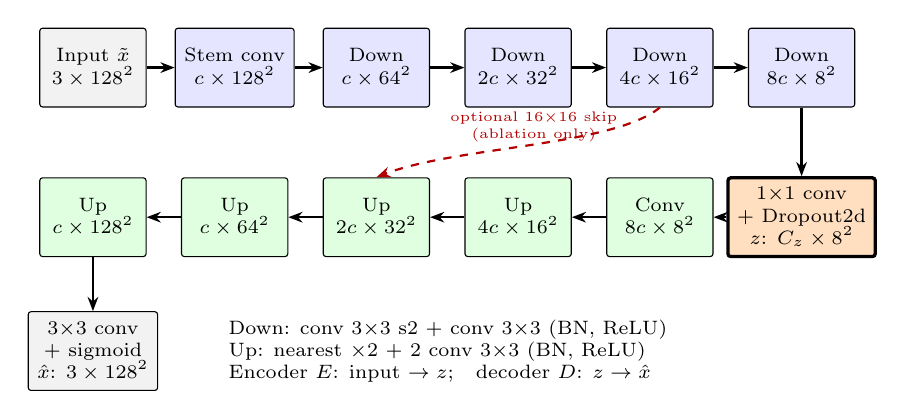
\begin{tikzpicture}[
    blk/.style={draw, rounded corners=1pt, minimum height=1.0cm, minimum width=1.35cm,
                align=center, font=\scriptsize},
    io/.style={blk, fill=gray!10},
    enc/.style={blk, fill=blue!10},
    dec/.style={blk, fill=green!12},
    lat/.style={blk, fill=orange!25, very thick},
    arr/.style={-{Stealth[length=1.8mm]}, thick}
  ]
  % Encoder row (left to right).
  \node[io]  (inp) at (0,0)    {Input $\tilde{x}$\\$3\times128^2$};
  \node[enc] (s)  at (1.8,0)  {Stem conv\\$c\times128^2$};
  \node[enc] (d1) at (3.6,0)  {Down\\$c\times64^2$};
  \node[enc] (d2) at (5.4,0)  {Down\\$2c\times32^2$};
  \node[enc] (d3) at (7.2,0)  {Down\\$4c\times16^2$};
  \node[enc] (d4) at (9.0,0)  {Down\\$8c\times8^2$};
  % Bottleneck.
  \node[lat] (z)  at (9.0,-1.9) {$1{\times}1$ conv\\+ Dropout2d\\$z$: $C_z\times8^2$};
  % Decoder row (right to left).
  \node[dec] (u0) at (7.2,-1.9) {Conv\\$8c\times8^2$};
  \node[dec] (u1) at (5.4,-1.9) {Up\\$4c\times16^2$};
  \node[dec] (u2) at (3.6,-1.9) {Up\\$2c\times32^2$};
  \node[dec] (u3) at (1.8,-1.9) {Up\\$c\times64^2$};
  \node[dec] (u4) at (0,-1.9)   {Up\\$c\times128^2$};
  \node[io]  (outp) at (0,-3.6)  {$3{\times}3$ conv\\+ sigmoid\\$\hat{x}$: $3\times128^2$};

  \draw[arr] (inp) -- (s);
  \draw[arr] (s) -- (d1);
  \draw[arr] (d1) -- (d2);
  \draw[arr] (d2) -- (d3);
  \draw[arr] (d3) -- (d4);
  \draw[arr] (d4) -- (z);
  \draw[arr] (z) -- (u0);
  \draw[arr] (u0) -- (u1);
  \draw[arr] (u1) -- (u2);
  \draw[arr] (u2) -- (u3);
  \draw[arr] (u3) -- (u4);
  \draw[arr] (u4) -- (outp);
  % Optional single skip at 16x16 (ablation only, off in the main model).
  \draw[arr, dashed, red!70!black] (d3.south) .. controls (6.6,-1.0) and (4.6,-1.0) .. (u2.north);
  \node[font=\tiny, red!70!black, align=center] at (5.6,-0.75) {optional 16$\times$16 skip\\(ablation only)};

  \node[font=\scriptsize, align=left, anchor=west] at (1.6,-3.6)
    {Down: conv $3{\times}3$ s2 + conv $3{\times}3$ (BN, ReLU)\\
     Up: nearest $\times2$ + 2 conv $3{\times}3$ (BN, ReLU)\\
     Encoder $E$: input $\rightarrow z$;\quad decoder $D$: $z \rightarrow \hat{x}$};
\end{tikzpicture}%
}
.
\resizebox{\columnwidth}{!}{%
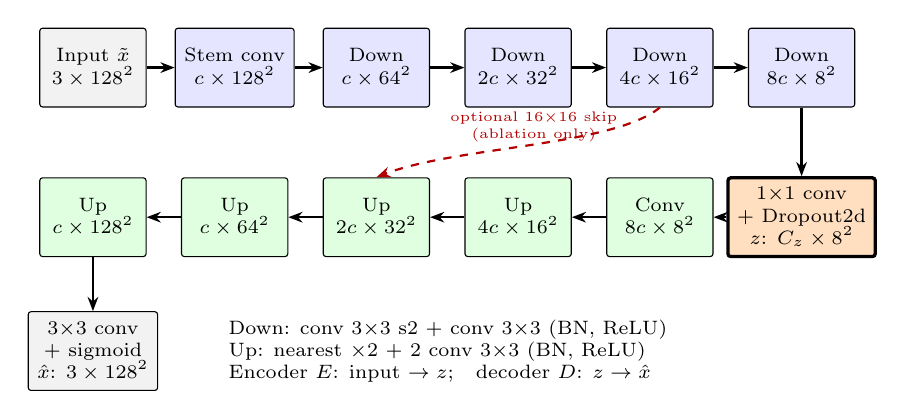
\begin{tikzpicture}[
    blk/.style={draw, rounded corners=1pt, minimum height=1.0cm, minimum width=1.35cm,
                align=center, font=\scriptsize},
    io/.style={blk, fill=gray!10},
    enc/.style={blk, fill=blue!10},
    dec/.style={blk, fill=green!12},
    lat/.style={blk, fill=orange!25, very thick},
    arr/.style={-{Stealth[length=1.8mm]}, thick}
  ]
  % Encoder row (left to right).
  \node[io]  (inp) at (0,0)    {Input $\tilde{x}$\\$3\times128^2$};
  \node[enc] (s)  at (1.8,0)  {Stem conv\\$c\times128^2$};
  \node[enc] (d1) at (3.6,0)  {Down\\$c\times64^2$};
  \node[enc] (d2) at (5.4,0)  {Down\\$2c\times32^2$};
  \node[enc] (d3) at (7.2,0)  {Down\\$4c\times16^2$};
  \node[enc] (d4) at (9.0,0)  {Down\\$8c\times8^2$};
  % Bottleneck.
  \node[lat] (z)  at (9.0,-1.9) {$1{\times}1$ conv\\+ Dropout2d\\$z$: $C_z\times8^2$};
  % Decoder row (right to left).
  \node[dec] (u0) at (7.2,-1.9) {Conv\\$8c\times8^2$};
  \node[dec] (u1) at (5.4,-1.9) {Up\\$4c\times16^2$};
  \node[dec] (u2) at (3.6,-1.9) {Up\\$2c\times32^2$};
  \node[dec] (u3) at (1.8,-1.9) {Up\\$c\times64^2$};
  \node[dec] (u4) at (0,-1.9)   {Up\\$c\times128^2$};
  \node[io]  (outp) at (0,-3.6)  {$3{\times}3$ conv\\+ sigmoid\\$\hat{x}$: $3\times128^2$};

  \draw[arr] (inp) -- (s);
  \draw[arr] (s) -- (d1);
  \draw[arr] (d1) -- (d2);
  \draw[arr] (d2) -- (d3);
  \draw[arr] (d3) -- (d4);
  \draw[arr] (d4) -- (z);
  \draw[arr] (z) -- (u0);
  \draw[arr] (u0) -- (u1);
  \draw[arr] (u1) -- (u2);
  \draw[arr] (u2) -- (u3);
  \draw[arr] (u3) -- (u4);
  \draw[arr] (u4) -- (outp);
  % Optional single skip at 16x16 (ablation only, off in the main model).
  \draw[arr, dashed, red!70!black] (d3.south) .. controls (6.6,-1.0) and (4.6,-1.0) .. (u2.north);
  \node[font=\tiny, red!70!black, align=center] at (5.6,-0.75) {optional 16$\times$16 skip\\(ablation only)};

  \node[font=\scriptsize, align=left, anchor=west] at (1.6,-3.6)
    {Down: conv $3{\times}3$ s2 + conv $3{\times}3$ (BN, ReLU)\\
     Up: nearest $\times2$ + 2 conv $3{\times}3$ (BN, ReLU)\\
     Encoder $E$: input $\rightarrow z$;\quad decoder $D$: $z \rightarrow \hat{x}$};
\end{tikzpicture}%
}
.
\resizebox{\columnwidth}{!}{%
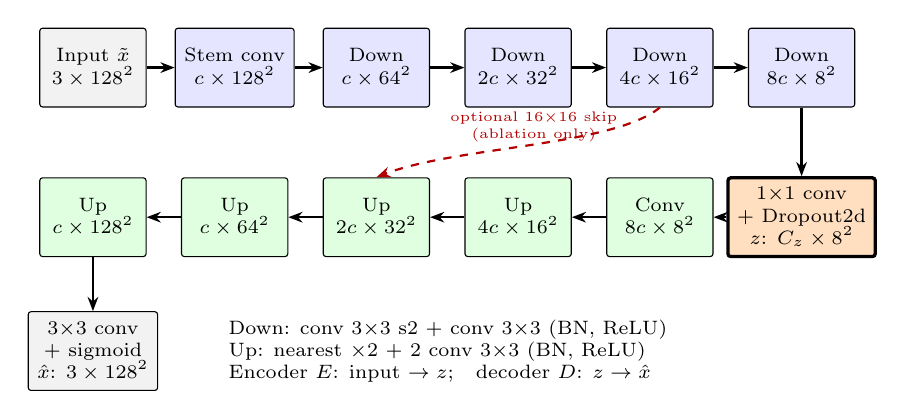
\begin{tikzpicture}[
    blk/.style={draw, rounded corners=1pt, minimum height=1.0cm, minimum width=1.35cm,
                align=center, font=\scriptsize},
    io/.style={blk, fill=gray!10},
    enc/.style={blk, fill=blue!10},
    dec/.style={blk, fill=green!12},
    lat/.style={blk, fill=orange!25, very thick},
    arr/.style={-{Stealth[length=1.8mm]}, thick}
  ]
  % Encoder row (left to right).
  \node[io]  (inp) at (0,0)    {Input $\tilde{x}$\\$3\times128^2$};
  \node[enc] (s)  at (1.8,0)  {Stem conv\\$c\times128^2$};
  \node[enc] (d1) at (3.6,0)  {Down\\$c\times64^2$};
  \node[enc] (d2) at (5.4,0)  {Down\\$2c\times32^2$};
  \node[enc] (d3) at (7.2,0)  {Down\\$4c\times16^2$};
  \node[enc] (d4) at (9.0,0)  {Down\\$8c\times8^2$};
  % Bottleneck.
  \node[lat] (z)  at (9.0,-1.9) {$1{\times}1$ conv\\+ Dropout2d\\$z$: $C_z\times8^2$};
  % Decoder row (right to left).
  \node[dec] (u0) at (7.2,-1.9) {Conv\\$8c\times8^2$};
  \node[dec] (u1) at (5.4,-1.9) {Up\\$4c\times16^2$};
  \node[dec] (u2) at (3.6,-1.9) {Up\\$2c\times32^2$};
  \node[dec] (u3) at (1.8,-1.9) {Up\\$c\times64^2$};
  \node[dec] (u4) at (0,-1.9)   {Up\\$c\times128^2$};
  \node[io]  (outp) at (0,-3.6)  {$3{\times}3$ conv\\+ sigmoid\\$\hat{x}$: $3\times128^2$};

  \draw[arr] (inp) -- (s);
  \draw[arr] (s) -- (d1);
  \draw[arr] (d1) -- (d2);
  \draw[arr] (d2) -- (d3);
  \draw[arr] (d3) -- (d4);
  \draw[arr] (d4) -- (z);
  \draw[arr] (z) -- (u0);
  \draw[arr] (u0) -- (u1);
  \draw[arr] (u1) -- (u2);
  \draw[arr] (u2) -- (u3);
  \draw[arr] (u3) -- (u4);
  \draw[arr] (u4) -- (outp);
  % Optional single skip at 16x16 (ablation only, off in the main model).
  \draw[arr, dashed, red!70!black] (d3.south) .. controls (6.6,-1.0) and (4.6,-1.0) .. (u2.north);
  \node[font=\tiny, red!70!black, align=center] at (5.6,-0.75) {optional 16$\times$16 skip\\(ablation only)};

  \node[font=\scriptsize, align=left, anchor=west] at (1.6,-3.6)
    {Down: conv $3{\times}3$ s2 + conv $3{\times}3$ (BN, ReLU)\\
     Up: nearest $\times2$ + 2 conv $3{\times}3$ (BN, ReLU)\\
     Encoder $E$: input $\rightarrow z$;\quad decoder $D$: $z \rightarrow \hat{x}$};
\end{tikzpicture}%
}

\caption{Task~1 autoencoder. $c$ is the base channel count and $C_z$ the
bottleneck channel count, both chosen by Optuna. The dashed skip exists only
in the ablation model.}
\label{fig:task1_arch}
\end{figure}

\emph{Form of the bottleneck.} Flattening to a single latent vector gives
the strongest compression but discards the spatial layout and requires a
large fully connected layer. We use a spatial bottleneck of $8\times8\times
C_z$; with $C_z\in\{16,32,64,128\}$ it holds 1,024 to 8,192 values, i.e.\
48, 24, 12 or 6 times fewer than the 49,152 input values, so the compression
ratio is an explicit, tuned quantity. Without skips, the decoder sees only
$z$; a unit test checks that \texttt{decode(encode(x))} equals
\texttt{forward(x)}, i.e.\ the output depends on the input only through the
bottleneck.

\emph{Decoder upsampling.} Transposed convolutions are learnable but prone
to checkerboard artefacts~\cite{odena2016deconvolution}; upsampling followed
by a convolution avoids them and also exports cleanly to ONNX, so we use the
latter.

\emph{Skip connections.} Full U-Net skips~\cite{ronneberger2015unet} would
let the network copy the input past the bottleneck, which the task forbids.
The main model therefore has none. To investigate the effect of a
\emph{limited} skip, the model optionally concatenates the $16\times16$
encoder feature ($4c$ channels) to the decoder at the same resolution; at
this resolution it cannot transmit pixel-level detail, but it does let
information bypass the $8\times8$ bottleneck. This variant is trained once
with the best configuration as an ablation (Section~\ref{sec:task1_ablation}).
For reference, the model has 1,865,891 parameters at $(c, C_z)=(32,32)$,
1,939,619 with the skip, 4,132,835 at $(48,32)$, 7,289,123 at $(64,32)$ and
7,780,739 at $(64,128)$.

\subsection{Loss function and metrics}
The model is trained with
\begin{equation}
\mathcal{L}_{\mathrm{rec}} = \alpha\,\mathcal{L}_{1}(x,\hat{x})
  + (1-\alpha)\bigl(1-\mathrm{SSIM}(x,\hat{x})\bigr),
\label{eq:rec_loss}
\end{equation}
where $x$ is the clean target. L1 rewards pixel accuracy and the SSIM
term~\cite{wang2004ssim} rewards preserved structure, edges and local
contrast. SSIM is computed with the \texttt{pytorch-msssim} implementation
(Gaussian window $11\times11$, $\sigma=1.5$, data range 1), both in the loss
and as a metric.
% TODO: justify the SSIM window choice after reading Wang et al. (decision log: "SSIM implementation and window size").
\TODO{Justify the SSIM implementation and window size (decision log entry
still open).}
We report PSNR, SSIM and L1 per image and average them per condition and
severity. PSNR uses a peak value of 1 and a mean squared error clamped at
$10^{-10}$, so an image returned unchanged scores a capped 100\,dB; because
such values would dominate an average that includes clean inputs, all
tables contain a separate ``corrupted'' row that excludes clean images. The
PSNR and SSIM of the corrupted input itself (the ``do nothing'' baseline)
are reported next to every restored value.

\subsection{Training procedure}
Training images are corrupted at runtime with the four conditions in equal
expectation (Section~\ref{sec:data}); the label is not given to the model.
We use Adam with a cosine-annealing learning-rate schedule over the run,
evaluate on the 2,944-item validation manifest after every epoch, and keep
the checkpoint of the epoch with the lowest validation objective
(Eq.~\eqref{eq:val_obj}). The final model is trained for 80 epochs; every
five epochs a grid of eight fixed corrupted validation images, their
restorations and targets is logged to W\&B.

\subsection{Optuna search design}
\label{sec:task1_optuna}
Trials train with different $\alpha$, so their own loss values are not
comparable: Optuna would favour whichever $\alpha$ makes the number small.
Every trial is therefore scored with one fixed validation objective that
combines reconstruction quality and structural similarity,
\begin{equation}
J = 0.8\,\mathcal{L}_{1} + 0.2\,(1-\mathrm{SSIM}),
\label{eq:val_obj}
\end{equation}
using the task's suggested starting weights, and the plain L1, PSNR and SSIM
are stored with every trial. A multi-objective search was considered but
returns a Pareto front instead of a single best trial. A trial with
$\alpha$ near 0.8 trains on almost exactly what is measured, which may
favour it slightly; we note this as a limitation. The study uses TPE (seed
42) and a median pruner (five start-up trials, three warm-up epochs); 30
trials of 10 epochs each are run. Table~\ref{tab:task1_space} gives the
search space.

\begin{table}[t]
\centering
\caption{Task 1 Optuna search space and selected configuration.}
\label{tab:task1_space}
\footnotesize
\begin{tabular}{llc}
\toprule
Hyperparameter & Range (scale) & Selected \\
\midrule
Learning rate & $10^{-4}$--$3\times10^{-3}$ (log) & \na \\
Batch size & \{32, 64, 128\} & \na \\
Bottleneck channels $C_z$ & \{16, 32, 64, 128\} & \na \\
Base channels $c$ & \{32, 48, 64\} & \na \\
Dropout (latent) & 0--0.3 (linear) & \na \\
Loss weight $\alpha$ & 0.5--0.95 (linear) & \na \\
\bottomrule
\end{tabular}
\\[3pt]
% TODO(results): fill "Selected" from configs/task1_udae_best.yaml and the study optuna_studies/task1_udae.db.
\TODO{Fill from \file{configs/task1_udae_best.yaml}.}
\end{table}

\subsection{Results}
\label{sec:task1_results}
% TODO(results): Optuna outcome for Task 1.
\TODO{Report the number of completed and pruned trials, the best trial
number, its objective, and the selected configuration (Table~\ref{tab:optuna_summary});
describe how the objective varied with $\alpha$ and $C_z$ (Optuna history and
parameter-importance plots, Fig.~\ref{fig:task1_optuna}).}

\begin{figure}[t]
\centering
\figOrTodo{figures/task1_udae_optuna.png}{\columnwidth}{Optuna optimisation history and
parameter importances for Task 1 (export from the study with optuna-dashboard
or optuna.visualization)}
\caption{Task 1 Optuna study.}
\label{fig:task1_optuna}
\end{figure}

\begin{figure}[t]
\centering
\figOrTodo{figures/task1_udae_curves.png}{\columnwidth}{Training loss and validation
objective/PSNR/SSIM per epoch of the final run (export from W\&B, group task1-udae, run final-task1\_udae)}
\caption{Task 1 training and validation curves.}
\label{fig:task1_curves}
\end{figure}

% TODO(results): interpret Fig. task1_curves (convergence, over-fitting, best epoch).
\TODO{Interpret the curves (Fig.~\ref{fig:task1_curves}): convergence, gap
between training and validation, epoch of the selected checkpoint.}

\begin{table}[t]
\centering
\caption{Task 1 test results per condition and severity (input = corrupted
image before restoration).}
\label{tab:task1_results}
\scriptsize
\setlength{\tabcolsep}{3pt}
\begin{tabular}{llrrrrr}
\toprule
Cond. & Sev. & In PSNR & PSNR & In SSIM & SSIM & L1 \\
\midrule
Clean & --   & \na & \na & \na & \na & \na \\
S\&P  & low  & \na & \na & \na & \na & \na \\
S\&P  & med. & \na & \na & \na & \na & \na \\
S\&P  & high & \na & \na & \na & \na & \na \\
Blur  & low  & \na & \na & \na & \na & \na \\
Blur  & med. & \na & \na & \na & \na & \na \\
Blur  & high & \na & \na & \na & \na & \na \\
Occl. & low  & \na & \na & \na & \na & \na \\
Occl. & med. & \na & \na & \na & \na & \na \\
Occl. & high & \na & \na & \na & \na & \na \\
\midrule
Corr. & all & \na & \na & \na & \na & \na \\
All       & all & \na & \na & \na & \na & \na \\
\bottomrule
\end{tabular}
\\[3pt]
% TODO(results): fill from report/results/task1_udae_test_metrics.csv.
\TODO{Fill from \file{report/results/task1_udae_test_metrics.csv}.}
\end{table}

\begin{figure}[t]
\centering
\figOrTodo{figures/task1_udae_psnr_bars.png}{\columnwidth}{PSNR before and after restoration per condition/severity}
\figOrTodo{figures/task1_udae_ssim_bars.png}{\columnwidth}{SSIM before and after restoration per condition/severity}
\caption{Task 1: input vs.\ restored PSNR (top) and SSIM (bottom) on the test manifest.}
\label{fig:task1_bars}
\end{figure}

% TODO(results): interpret Table task1_results and Fig. task1_bars.
\TODO{Interpret Table~\ref{tab:task1_results} and Fig.~\ref{fig:task1_bars}:
which corruption and severity is restored best/worst, how restoration
compares with the input baseline, and whether clean inputs are degraded by
passing through the autoencoder.}

\begin{figure*}[t]
\centering
\figOrTodo{figures/task1_udae_examples.png}{0.85\textwidth}{Twelve representative test
examples: clean target, corrupted input, restored output, absolute error map (median-PSNR item of every condition/severity, plus two extra clean items)}
\caption{Task 1 representative test examples. Columns: clean target,
corrupted input, restored output, absolute error (fixed colour scale 0--0.5).}
\label{fig:task1_examples}
\end{figure*}

% TODO(results): discuss the twelve examples in Fig. task1_examples.
\TODO{Discuss the twelve examples of Fig.~\ref{fig:task1_examples}: where
the error maps concentrate (edges, texture, occluded regions).}

\subsection{Skip-connection ablation}
\label{sec:task1_ablation}
% TODO(results): run train_udae --mode final --skip, then eval_udae --name task1_udae_skip.
\TODO{Train \file{python -m src.training.train_udae --mode final --skip} and
evaluate with \file{python -m src.evaluation.eval_udae --name task1_udae_skip};
fill Table~\ref{tab:task1_ablation} from \file{report/results/task1_udae_skip_test_metrics.csv}
and state what the limited skip changes and whether it weakens the bottleneck.}

\begin{table}[t]
\centering
\caption{Ablation: main model (no skip) vs.\ one $16\times16$ skip, test set.}
\label{tab:task1_ablation}
\footnotesize
\begin{tabular}{lrrrr}
\toprule
 & \multicolumn{2}{c}{No skip} & \multicolumn{2}{c}{$16\times16$ skip} \\
\cmidrule(lr){2-3}\cmidrule(lr){4-5}
Condition & PSNR & SSIM & PSNR & SSIM \\
\midrule
Clean           & \na & \na & \na & \na \\
Salt-and-pepper & \na & \na & \na & \na \\
Blur            & \na & \na & \na & \na \\
Occlusion       & \na & \na & \na & \na \\
Corrupted (all) & \na & \na & \na & \na \\
\bottomrule
\end{tabular}
\end{table}

\subsection{Failure cases}
\begin{figure*}[t]
\centering
\figOrTodo{figures/task1_udae_failures.png}{0.85\textwidth}{Four failure cases: the lowest-SSIM test item of each condition}
\caption{Task 1 failure cases (lowest SSIM per condition).}
\label{fig:task1_failures}
\end{figure*}
% TODO(results): discuss the four failure cases.
\TODO{Explain each of the four failures in Fig.~\ref{fig:task1_failures} and
why it occurred (e.g.\ occluded content that is not recoverable from the
input, dense noise on fine texture).}

\subsection{Discussion}
% TODO(results): Task 1 discussion.
\TODO{Discuss what the results show about a single shared representation for
all conditions, the role of the selected $\alpha$ and $C_z$, and how this
motivated Tasks 2 and 3.}

% =====================================================================
\section{Task 2: Classification and Hard-Routed Specialists}
\label{sec:task2}

\subsection{Corruption classifier}
The classifier $C$ (Fig.~\ref{fig:task2_arch}) has four blocks of two
$3\times3$ convolutions with batch normalisation and ReLU followed by
$2\times2$ max-pooling ($128\to64\to32\to16\to8$), then global average
pooling, dropout and a linear layer to four logits. The channel widths are
one of three presets tuned by Optuna: small (16--128, 294,516 parameters),
medium (32--256, 1,174,244) and large (48--384, 2,639,188). We considered
downsampling early (a stride-2 first layer, or a pretrained ImageNet network
on resized input), but the evidence that separates a clean image from a
mildly blurred or lightly noisy one lies in single pixels and fine edges,
which early downsampling removes; the first block therefore runs at full
resolution. The network outputs raw logits rather than probabilities,
because cross-entropy expects logits and the same network later becomes the
Task~3 gate, which applies its own tempered softmax. The class probabilities
are $p=\mathrm{softmax}(C(\tilde{x}))$ and the predicted class is
$r=\arg\max_k p_k$.

\begin{figure}[t]
\centering
% Task 2: classifier followed by hard routing (src/models/hard_router.py).
% Included from main.tex with % Task 2: classifier followed by hard routing (src/models/hard_router.py).
% Included from main.tex with % Task 2: classifier followed by hard routing (src/models/hard_router.py).
% Included from main.tex with \input{figures/tikz/task2_hard_routing}.
\resizebox{\columnwidth}{!}{%
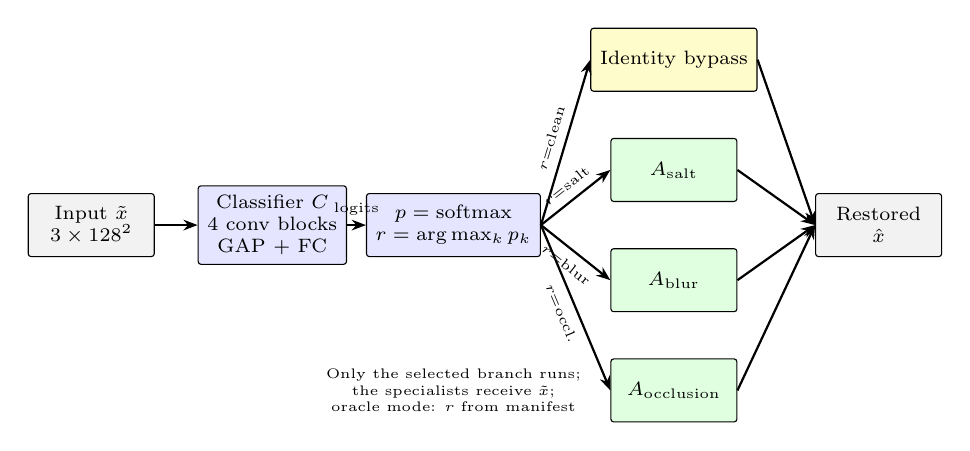
\begin{tikzpicture}[
    blk/.style={draw, rounded corners=1pt, minimum height=0.8cm, minimum width=1.6cm,
                align=center, font=\scriptsize},
    io/.style={blk, fill=gray!10},
    cls/.style={blk, fill=blue!10},
    exp/.style={blk, fill=green!12},
    idn/.style={blk, fill=yellow!20},
    arr/.style={-{Stealth[length=1.8mm]}, thick}
  ]
  \node[io]  (inp)  at (0,0)   {Input $\tilde{x}$\\$3\times128^2$};
  \node[cls] (c)   at (2.3,0) {Classifier $C$\\4 conv blocks\\GAP + FC};
  \node[cls] (r)   at (4.6,0) {$p=\mathrm{softmax}$\\$r=\arg\max_k p_k$};

  \node[idn] (b0) at (7.4,2.1)  {Identity bypass};
  \node[exp] (b1) at (7.4,0.7)  {$A_{\mathrm{salt}}$};
  \node[exp] (b2) at (7.4,-0.7) {$A_{\mathrm{blur}}$};
  \node[exp] (b3) at (7.4,-2.1) {$A_{\mathrm{occlusion}}$};

  \node[io]  (outp) at (10.0,0) {Restored\\$\hat{x}$};

  \draw[arr] (inp) -- (c);
  \draw[arr] (c) -- node[above, font=\tiny] {logits} (r);
  \draw[arr] (r.east) -- node[above, sloped, font=\tiny] {$r$=clean} (b0.west);
  \draw[arr] (r.east) -- node[above, sloped, font=\tiny] {$r$=salt} (b1.west);
  \draw[arr] (r.east) -- node[below, sloped, font=\tiny] {$r$=blur} (b2.west);
  \draw[arr] (r.east) -- node[below, sloped, font=\tiny] {$r$=occl.} (b3.west);
  \draw[arr] (b0.east) -- (outp.west);
  \draw[arr] (b1.east) -- (outp.west);
  \draw[arr] (b2.east) -- (outp.west);
  \draw[arr] (b3.east) -- (outp.west);

  \node[font=\tiny, align=center] at (4.6,-2.1)
    {Only the selected branch runs;\\the specialists receive $\tilde{x}$;\\oracle mode: $r$ from manifest};
\end{tikzpicture}%
}
.
\resizebox{\columnwidth}{!}{%
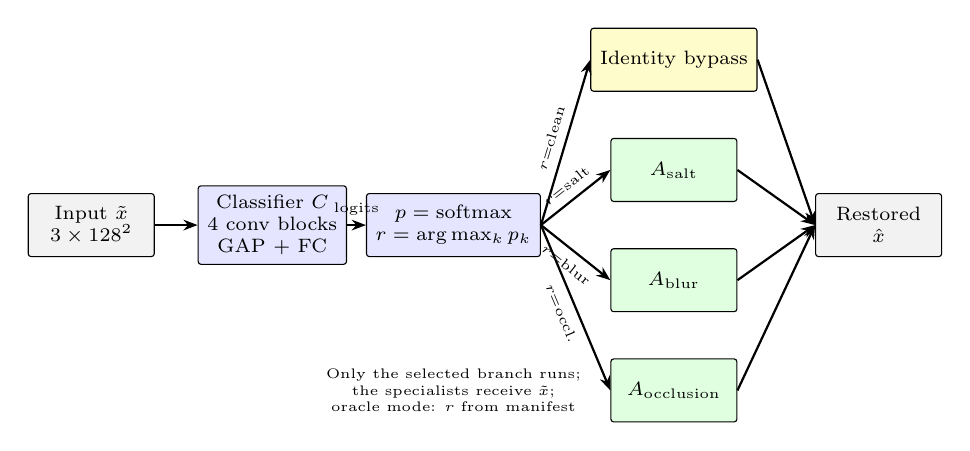
\begin{tikzpicture}[
    blk/.style={draw, rounded corners=1pt, minimum height=0.8cm, minimum width=1.6cm,
                align=center, font=\scriptsize},
    io/.style={blk, fill=gray!10},
    cls/.style={blk, fill=blue!10},
    exp/.style={blk, fill=green!12},
    idn/.style={blk, fill=yellow!20},
    arr/.style={-{Stealth[length=1.8mm]}, thick}
  ]
  \node[io]  (inp)  at (0,0)   {Input $\tilde{x}$\\$3\times128^2$};
  \node[cls] (c)   at (2.3,0) {Classifier $C$\\4 conv blocks\\GAP + FC};
  \node[cls] (r)   at (4.6,0) {$p=\mathrm{softmax}$\\$r=\arg\max_k p_k$};

  \node[idn] (b0) at (7.4,2.1)  {Identity bypass};
  \node[exp] (b1) at (7.4,0.7)  {$A_{\mathrm{salt}}$};
  \node[exp] (b2) at (7.4,-0.7) {$A_{\mathrm{blur}}$};
  \node[exp] (b3) at (7.4,-2.1) {$A_{\mathrm{occlusion}}$};

  \node[io]  (outp) at (10.0,0) {Restored\\$\hat{x}$};

  \draw[arr] (inp) -- (c);
  \draw[arr] (c) -- node[above, font=\tiny] {logits} (r);
  \draw[arr] (r.east) -- node[above, sloped, font=\tiny] {$r$=clean} (b0.west);
  \draw[arr] (r.east) -- node[above, sloped, font=\tiny] {$r$=salt} (b1.west);
  \draw[arr] (r.east) -- node[below, sloped, font=\tiny] {$r$=blur} (b2.west);
  \draw[arr] (r.east) -- node[below, sloped, font=\tiny] {$r$=occl.} (b3.west);
  \draw[arr] (b0.east) -- (outp.west);
  \draw[arr] (b1.east) -- (outp.west);
  \draw[arr] (b2.east) -- (outp.west);
  \draw[arr] (b3.east) -- (outp.west);

  \node[font=\tiny, align=center] at (4.6,-2.1)
    {Only the selected branch runs;\\the specialists receive $\tilde{x}$;\\oracle mode: $r$ from manifest};
\end{tikzpicture}%
}
.
\resizebox{\columnwidth}{!}{%
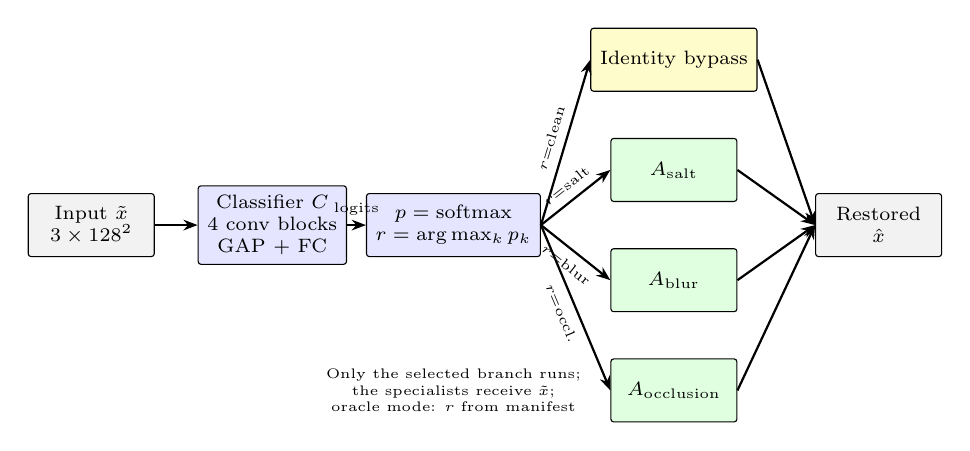
\begin{tikzpicture}[
    blk/.style={draw, rounded corners=1pt, minimum height=0.8cm, minimum width=1.6cm,
                align=center, font=\scriptsize},
    io/.style={blk, fill=gray!10},
    cls/.style={blk, fill=blue!10},
    exp/.style={blk, fill=green!12},
    idn/.style={blk, fill=yellow!20},
    arr/.style={-{Stealth[length=1.8mm]}, thick}
  ]
  \node[io]  (inp)  at (0,0)   {Input $\tilde{x}$\\$3\times128^2$};
  \node[cls] (c)   at (2.3,0) {Classifier $C$\\4 conv blocks\\GAP + FC};
  \node[cls] (r)   at (4.6,0) {$p=\mathrm{softmax}$\\$r=\arg\max_k p_k$};

  \node[idn] (b0) at (7.4,2.1)  {Identity bypass};
  \node[exp] (b1) at (7.4,0.7)  {$A_{\mathrm{salt}}$};
  \node[exp] (b2) at (7.4,-0.7) {$A_{\mathrm{blur}}$};
  \node[exp] (b3) at (7.4,-2.1) {$A_{\mathrm{occlusion}}$};

  \node[io]  (outp) at (10.0,0) {Restored\\$\hat{x}$};

  \draw[arr] (inp) -- (c);
  \draw[arr] (c) -- node[above, font=\tiny] {logits} (r);
  \draw[arr] (r.east) -- node[above, sloped, font=\tiny] {$r$=clean} (b0.west);
  \draw[arr] (r.east) -- node[above, sloped, font=\tiny] {$r$=salt} (b1.west);
  \draw[arr] (r.east) -- node[below, sloped, font=\tiny] {$r$=blur} (b2.west);
  \draw[arr] (r.east) -- node[below, sloped, font=\tiny] {$r$=occl.} (b3.west);
  \draw[arr] (b0.east) -- (outp.west);
  \draw[arr] (b1.east) -- (outp.west);
  \draw[arr] (b2.east) -- (outp.west);
  \draw[arr] (b3.east) -- (outp.west);

  \node[font=\tiny, align=center] at (4.6,-2.1)
    {Only the selected branch runs;\\the specialists receive $\tilde{x}$;\\oracle mode: $r$ from manifest};
\end{tikzpicture}%
}

\caption{Task~2 hard routing: the classifier selects exactly one branch;
clean inputs bypass all experts.}
\label{fig:task2_arch}
\end{figure}

\subsection{Balanced batches, loss and training}
The training batches must not favour any class. Drawing a random condition
per image, or using a weighted sampler, is balanced only in expectation: a
batch of 32 can easily contain 4 images of one class and 12 of another. We
instead assign labels by batch position ($0,1,2,3,0,1,\dots$), shuffle the
assignment, and corrupt each image according to its label; batch sizes are
multiples of four and the last incomplete batch is dropped, so every batch
contains exactly 25\% of each class. Tests confirm exact counts of $B/4$ per
class for batch sizes 4, 8 and 64 and over a full epoch.

The classifier is trained with multiclass cross-entropy and
AdamW~\cite{loshchilov2019decoupled} with a cosine schedule, for 40 epochs in
the final run. The checkpoint is chosen by validation macro-F1, with ties
broken by the lower validation cross-entropy.

\subsection{Classifier Optuna search}
The search maximises validation macro-F1 on the balanced validation
manifest. On a perfectly balanced set accuracy would rank models almost
identically, but macro-F1 is a required metric and penalises a model that
sacrifices one class; validation cross-entropy is smoother but rewards
confident probabilities rather than correct decisions, so it is only logged
and used as the tie-breaker. TPE and a median pruner (five start-up trials,
three warm-up epochs) run 25 trials of 8 epochs. Table~\ref{tab:task2_cls_space}
gives the search space.

\begin{table}[t]
\centering
\caption{Task 2 classifier search space and selected configuration.}
\label{tab:task2_cls_space}
\footnotesize
\begin{tabular}{llc}
\toprule
Hyperparameter & Range (scale) & Selected \\
\midrule
Learning rate & $10^{-4}$--$3\times10^{-3}$ (log) & \na \\
Batch size & \{32, 64, 128\} & \na \\
Channel preset & \{small, medium, large\} & \na \\
Dropout & 0--0.5 (linear) & \na \\
Weight decay (AdamW) & $10^{-6}$--$10^{-3}$ (log) & \na \\
\bottomrule
\end{tabular}
\\[3pt]
% TODO(results): fill from configs/task2_classifier_best.yaml.
\TODO{Fill from \file{configs/task2_classifier_best.yaml}.}
\end{table}

\subsection{Specialist autoencoders}
The three specialists $A_{\mathrm{salt}}$, $A_{\mathrm{blur}}$ and
$A_{\mathrm{occlusion}}$ use the Task~1 architecture without dropout and
the same clean targets. Each is trained only on its own corruption type
(sampled at runtime from the training ranges) and validated only on the 736
validation-manifest items of that type, with the loss of
Eq.~\eqref{eq:rec_loss}, Adam and a cosine schedule (60 epochs in the final
run). The parameters of the three are independent.

Three separate searches would give the most tailored settings at three
times the cost; tuning one proxy model trained on all three corruptions is
cheaper but tunes a model that is never used. We use one shared Optuna study
that scores the three real specialists: in each trial they are trained side
by side (one epoch each in turn), and the trial's value is the mean of their
fixed validation objectives (Eq.~\eqref{eq:val_obj}), which also allows
per-epoch pruning on the mean. The best shared configuration is then used to
train the three specialists independently, each with its own W\&B run and
checkpoint. The study runs 20 trials of 8 epochs (Table~\ref{tab:task2_spec_space}).

\begin{table}[t]
\centering
\caption{Task 2 specialist (shared) search space and selected configuration.
Dropout is fixed at 0.}
\label{tab:task2_spec_space}
\footnotesize
\begin{tabular}{llc}
\toprule
Hyperparameter & Range (scale) & Selected \\
\midrule
Learning rate & $10^{-4}$--$3\times10^{-3}$ (log) & \na \\
Batch size & \{32, 64, 128\} & \na \\
Bottleneck channels $C_z$ & \{16, 32, 64, 128\} & \na \\
Base channels $c$ & \{32, 48, 64\} & \na \\
L1 weight $\alpha$ & 0.5--0.95 (linear) & \na \\
\bottomrule
\end{tabular}
\\[3pt]
% TODO(results): fill from configs/task2_specialists_best.yaml.
\TODO{Fill from \file{configs/task2_specialists_best.yaml}.}
\end{table}

\subsection{Hard routing and evaluation modes}
At inference the classifier chooses the branch,
\begin{equation}
\hat{x} =
\begin{cases}
\tilde{x}, & r=\text{clean},\\
A_{\mathrm{salt}}(\tilde{x}), & r=\text{salt},\\
A_{\mathrm{blur}}(\tilde{x}), & r=\text{blur},\\
A_{\mathrm{occlusion}}(\tilde{x}), & r=\text{occlusion}.
\end{cases}
\label{eq:hard_routing}
\end{equation}
Running all three experts and selecting one output afterwards would triple
the work and pass clean images through an expert, contrary to the identity
bypass. Our router instead runs each expert only on the images routed to it
and returns clean-routed images unchanged; tests confirm that these images
are bit-identical to the input and that an expert is not called when nothing
is routed to it. The system is evaluated on the test manifest in
\emph{oracle} mode (the manifest label selects the branch, measuring the
specialists) and in \emph{predicted} mode (the classifier selects it,
measuring the operational system). Misrouted images are tabulated by (true
class, chosen branch) with their PSNR and SSIM loss relative to oracle
routing; for clean images the SSIM loss is the more meaningful number,
because the oracle output has the capped PSNR. The six misrouted images with
the largest PSNR loss are shown.

\subsection{Results}
% TODO(results): Task 2 Optuna outcomes for both studies.
\TODO{Report completed/pruned trials and the best trial of both Task 2
studies (Table~\ref{tab:optuna_summary}) and interpret the
selected configurations and the training curves (Fig.~\ref{fig:task2_curves}).}

\begin{figure}[t]
\centering
\figOrTodo{figures/task2_curves.png}{\columnwidth}{Classifier training loss/accuracy and
validation macro-F1/cross-entropy per epoch, and specialist validation objectives (export from W\&B groups task2-classifier and task2-specialists)}
\caption{Task 2 training and validation curves.}
\label{fig:task2_curves}
\end{figure}

\begin{table}[t]
\centering
\caption{Task 2 classifier on the test manifest (36,690 items).}
\label{tab:task2_cls_overall}
\footnotesize
\begin{tabular}{lcccc}
\toprule
 & Accuracy & Macro-P & Macro-R & Macro-F1 \\
\midrule
Test & \na & \na & \na & \na \\
\bottomrule
\end{tabular}
\\[6pt]
\begin{tabular}{lccc}
\toprule
Class & Precision & Recall & F1 \\
\midrule
Clean           & \na & \na & \na \\
Salt-and-pepper & \na & \na & \na \\
Blur            & \na & \na & \na \\
Occlusion       & \na & \na & \na \\
\bottomrule
\end{tabular}
\\[3pt]
% TODO(results): fill from report/results/task2_classifier_per_class.csv (eval_task2 also prints the overall numbers).
\TODO{Fill from \file{report/results/task2_classifier_per_class.csv}.}
\end{table}

\begin{table}[t]
\centering
\caption{Task 2 classifier accuracy per test severity.}
\label{tab:task2_cls_severity}
\footnotesize
\begin{tabular}{lcccc}
\toprule
Condition & none & low & medium & high \\
\midrule
Clean           & \na & --  & --  & --  \\
Salt-and-pepper & --  & \na & \na & \na \\
Blur            & --  & \na & \na & \na \\
Occlusion       & --  & \na & \na & \na \\
\bottomrule
\end{tabular}
\\[3pt]
% TODO(results): fill from report/results/task2_classifier_by_severity.csv.
\TODO{Fill from \file{report/results/task2_classifier_by_severity.csv}.}
\end{table}

\begin{figure}[t]
\centering
\figOrTodo{figures/task2_test_confusion.png}{0.8\columnwidth}{Row-normalised 4-class test confusion matrix}
\caption{Task 2 classifier: normalised confusion matrix on the test manifest.
The validation matrix of the selected epoch is in
\file{figures/task2_classifier_val_confusion.png}.}
\label{fig:task2_confusion}
\end{figure}

% TODO(results): interpret the classifier tables and confusion matrix.
\TODO{Interpret Tables~\ref{tab:task2_cls_overall}--\ref{tab:task2_cls_severity}
and Fig.~\ref{fig:task2_confusion}: which classes are confused and at which
severities (the clean vs.\ low-blur pair was expected to be the hardest;
confirm or refute).}

\begin{table}[t]
\centering
\caption{Task 2 restoration on the test manifest: oracle vs.\ predicted routing.}
\label{tab:task2_restoration}
\scriptsize
\setlength{\tabcolsep}{3pt}
\begin{tabular}{llrrrrr}
\toprule
 & & & \multicolumn{2}{c}{PSNR} & \multicolumn{2}{c}{SSIM} \\
\cmidrule(lr){4-5}\cmidrule(lr){6-7}
Cond. & Sev. & In PSNR & Oracle & Pred. & Oracle & Pred. \\
\midrule
Clean & --   & \na & \na & \na & \na & \na \\
S\&P  & low  & \na & \na & \na & \na & \na \\
S\&P  & med. & \na & \na & \na & \na & \na \\
S\&P  & high & \na & \na & \na & \na & \na \\
Blur  & low  & \na & \na & \na & \na & \na \\
Blur  & med. & \na & \na & \na & \na & \na \\
Blur  & high & \na & \na & \na & \na & \na \\
Occl. & low  & \na & \na & \na & \na & \na \\
Occl. & med. & \na & \na & \na & \na & \na \\
Occl. & high & \na & \na & \na & \na & \na \\
\midrule
Corr. & all & \na & \na & \na & \na & \na \\
All       & all & \na & \na & \na & \na & \na \\
\bottomrule
\end{tabular}
\\[3pt]
% TODO(results): fill from report/results/task2_oracle_test_metrics.csv and task2_predicted_test_metrics.csv.
\TODO{Fill from \file{report/results/task2_oracle_test_metrics.csv} and
\file{task2_predicted_test_metrics.csv}.}
\end{table}

\begin{figure}[t]
\centering
\figOrTodo{figures/task2_predicted_psnr_bars.png}{\columnwidth}{Predicted-routing PSNR before and after restoration}
\caption{Task 2 (predicted routing): input vs.\ restored PSNR per condition and severity.}
\label{fig:task2_bars}
\end{figure}

\begin{figure*}[t]
\centering
\figOrTodo{figures/task2_examples.png}{0.85\textwidth}{Twelve representative predicted-routing test examples with routed expert and error maps}
\caption{Task 2 representative examples (predicted routing): clean target,
corrupted input, restored output, absolute error; row labels give the chosen expert.}
\label{fig:task2_examples}
\end{figure*}

% TODO(results): interpret oracle vs. predicted.
\TODO{Interpret Table~\ref{tab:task2_restoration}, Fig.~\ref{fig:task2_bars}
and Fig.~\ref{fig:task2_examples}: the specialists' quality (oracle), the
gap to predicted routing and where it arises, and the comparison with Task~1.}

\subsection{Failure cases caused by misrouting}
\begin{table}[t]
\centering
\caption{Misrouted test images by true class and chosen branch, with the
mean loss relative to oracle routing.}
\label{tab:task2_misrouting}
\footnotesize
\begin{tabular}{llrrr}
\toprule
True class & Routed to & Count & PSNR loss & SSIM loss \\
\midrule
\na & \na & \na & \na & \na \\
\na & \na & \na & \na & \na \\
\na & \na & \na & \na & \na \\
\bottomrule
\end{tabular}
\\[3pt]
% TODO(results): one row per (true, routed_to) pair in report/results/task2_misrouting.csv.
\TODO{One row per pair in \file{report/results/task2_misrouting.csv}.}
\end{table}

\begin{figure*}[t]
\centering
\figOrTodo{figures/task2_misrouted.png}{0.85\textwidth}{The six misrouted test images with the largest PSNR loss vs.\ oracle routing}
\caption{Task 2 failures caused by classifier errors: the six misrouted images
with the largest PSNR loss relative to oracle routing.}
\label{fig:task2_misrouted}
\end{figure*}

% TODO(results): discuss misrouting failures.
\TODO{Discuss Table~\ref{tab:task2_misrouting} and Fig.~\ref{fig:task2_misrouted}:
which errors are frequent, which are costly, and why the classifier failed
on these inputs.}

\subsection{Discussion}
% TODO(results): Task 2 discussion.
\TODO{Discuss specialisation vs.\ a universal model, and the cost of hard
decisions near class boundaries (motivation for Task~3).}

% =====================================================================
\section{Task 3: Soft Mixture-of-Experts}
\label{sec:task3}

\subsection{Architecture and initialisation}
The soft system (Fig.~\ref{fig:task3_arch}) contains a gate $G$, an identity
branch and the three Task~2 experts. The gate produces
\begin{equation}
w = \mathrm{softmax}\!\left(G(\tilde{x})/\tau\right),\quad
w=[w_0,w_1,w_2,w_3],
\end{equation}
and the output is the convex combination
\begin{equation}
\hat{x} = w_0\tilde{x} + w_1A_{\mathrm{salt}}(\tilde{x})
 + w_2A_{\mathrm{blur}}(\tilde{x}) + w_3A_{\mathrm{occlusion}}(\tilde{x}).
\label{eq:moe}
\end{equation}
Every branch processes every image, which is required for the gradient of
every weight and keeps the exported graph free of data-dependent branches;
a sparse top-$k$ mixture~\cite{shazeer2017outrageously} would be cheaper but
would no longer be the weighted sum of Eq.~\eqref{eq:moe}. Since each expert
ends in a sigmoid, the identity branch lies in $[0,1]$ and the weights are
non-negative and sum to one, $\hat{x}$ stays in $[0,1]$ without clamping.
The temperature $\tau$ is a fixed hyperparameter of each run, stored in the
model so that it is saved with the weights and baked into the ONNX graph.

Training does not start from random components: the gate is the trained
Task~2 classifier network and the experts are the three trained
specialists. A random gate would hand the experts meaningless mixtures to
learn from.

\begin{figure}[t]
\centering
% Task 3: soft mixture-of-experts (src/models/soft_moe.py).
% Included from main.tex with % Task 3: soft mixture-of-experts (src/models/soft_moe.py).
% Included from main.tex with % Task 3: soft mixture-of-experts (src/models/soft_moe.py).
% Included from main.tex with \input{figures/tikz/task3_soft_moe}.
\resizebox{\columnwidth}{!}{%
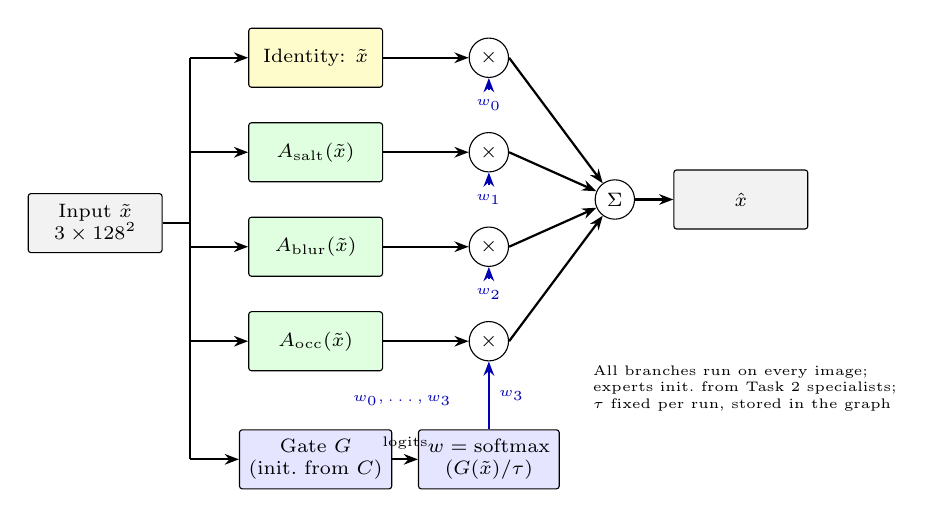
\begin{tikzpicture}[
    blk/.style={draw, rounded corners=1pt, minimum height=0.75cm, minimum width=1.7cm,
                align=center, font=\scriptsize},
    io/.style={blk, fill=gray!10},
    gate/.style={blk, fill=blue!10},
    exp/.style={blk, fill=green!12},
    idn/.style={blk, fill=yellow!20},
    op/.style={draw, circle, inner sep=1pt, minimum size=0.5cm, font=\scriptsize},
    arr/.style={-{Stealth[length=1.8mm]}, thick}
  ]
  \node[io]  (inp) at (0,0) {Input $\tilde{x}$\\$3\times128^2$};

  \node[idn] (b0) at (2.8,2.1)  {Identity: $\tilde{x}$};
  \node[exp] (b1) at (2.8,0.9)  {$A_{\mathrm{salt}}(\tilde{x})$};
  \node[exp] (b2) at (2.8,-0.3) {$A_{\mathrm{blur}}(\tilde{x})$};
  \node[exp] (b3) at (2.8,-1.5) {$A_{\mathrm{occ}}(\tilde{x})$};

  \node[op] (m0) at (5.0,2.1)  {$\times$};
  \node[op] (m1) at (5.0,0.9)  {$\times$};
  \node[op] (m2) at (5.0,-0.3) {$\times$};
  \node[op] (m3) at (5.0,-1.5) {$\times$};

  \node[op] (sum) at (6.6,0.3) {$\Sigma$};
  \node[io] (outp) at (8.2,0.3) {$\hat{x}$};

  \node[gate] (g)  at (2.8,-3.0) {Gate $G$\\(init.\ from $C$)};
  \node[gate] (sm) at (5.0,-3.0) {$w=\mathrm{softmax}$\\$(G(\tilde{x})/\tau)$};

  % Input to every branch and to the gate.
  \draw[thick] (inp.east) -- (1.2,0);
  \draw[thick] (1.2,2.1) -- (1.2,-3.0);
  \draw[arr] (1.2,2.1)  -- (b0.west);
  \draw[arr] (1.2,0.9)  -- (b1.west);
  \draw[arr] (1.2,-0.3) -- (b2.west);
  \draw[arr] (1.2,-1.5) -- (b3.west);
  \draw[arr] (1.2,-3.0) -- (g.west);

  \draw[arr] (b0) -- (m0);
  \draw[arr] (b1) -- (m1);
  \draw[arr] (b2) -- (m2);
  \draw[arr] (b3) -- (m3);

  \draw[arr] (g) -- node[above, font=\tiny] {logits} (sm);
  % Each multiplier receives its routing weight from below (blue labels);
  % the weights are the outputs of the softmax node.
  \node[font=\tiny, text=blue!70!black] (w0) at (5.0,1.5)  {$w_0$};
  \node[font=\tiny, text=blue!70!black] (w1) at (5.0,0.3)  {$w_1$};
  \node[font=\tiny, text=blue!70!black] (w2) at (5.0,-0.9) {$w_2$};
  \draw[arr, blue!70!black] (w0) -- (m0);
  \draw[arr, blue!70!black] (w1) -- (m1);
  \draw[arr, blue!70!black] (w2) -- (m2);
  \draw[arr, blue!70!black] (sm) -- node[right, font=\tiny] {$w_3$} (m3);
  \node[font=\tiny, text=blue!70!black, align=center] at (3.9,-2.25) {$w_0,\dots,w_3$};

  \draw[arr] (m0.east) -- (sum);
  \draw[arr] (m1.east) -- (sum);
  \draw[arr] (m2.east) -- (sum);
  \draw[arr] (m3.east) -- (sum);
  \draw[arr] (sum) -- (outp);

  \node[font=\tiny, align=left, anchor=west] at (6.2,-2.1)
    {All branches run on every image;\\experts init.\ from Task 2 specialists;\\$\tau$ fixed per run, stored in the graph};
\end{tikzpicture}%
}
.
\resizebox{\columnwidth}{!}{%
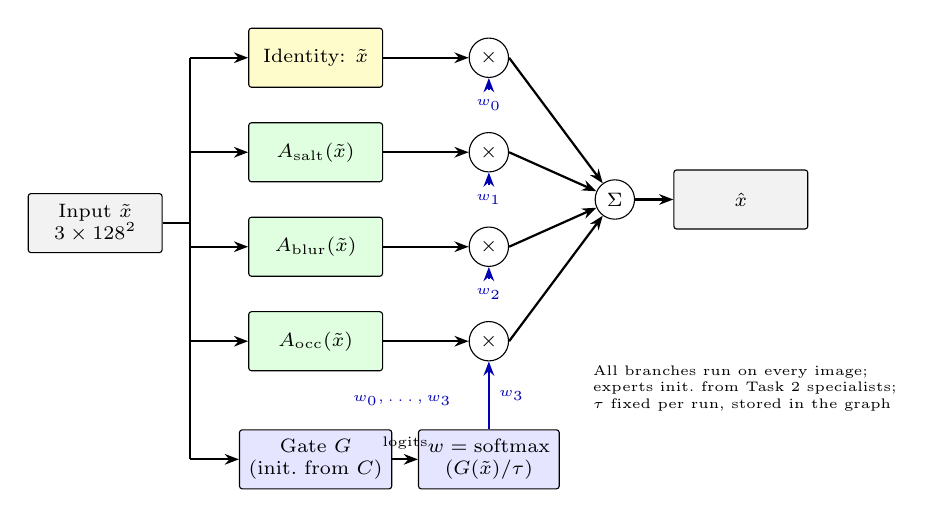
\begin{tikzpicture}[
    blk/.style={draw, rounded corners=1pt, minimum height=0.75cm, minimum width=1.7cm,
                align=center, font=\scriptsize},
    io/.style={blk, fill=gray!10},
    gate/.style={blk, fill=blue!10},
    exp/.style={blk, fill=green!12},
    idn/.style={blk, fill=yellow!20},
    op/.style={draw, circle, inner sep=1pt, minimum size=0.5cm, font=\scriptsize},
    arr/.style={-{Stealth[length=1.8mm]}, thick}
  ]
  \node[io]  (inp) at (0,0) {Input $\tilde{x}$\\$3\times128^2$};

  \node[idn] (b0) at (2.8,2.1)  {Identity: $\tilde{x}$};
  \node[exp] (b1) at (2.8,0.9)  {$A_{\mathrm{salt}}(\tilde{x})$};
  \node[exp] (b2) at (2.8,-0.3) {$A_{\mathrm{blur}}(\tilde{x})$};
  \node[exp] (b3) at (2.8,-1.5) {$A_{\mathrm{occ}}(\tilde{x})$};

  \node[op] (m0) at (5.0,2.1)  {$\times$};
  \node[op] (m1) at (5.0,0.9)  {$\times$};
  \node[op] (m2) at (5.0,-0.3) {$\times$};
  \node[op] (m3) at (5.0,-1.5) {$\times$};

  \node[op] (sum) at (6.6,0.3) {$\Sigma$};
  \node[io] (outp) at (8.2,0.3) {$\hat{x}$};

  \node[gate] (g)  at (2.8,-3.0) {Gate $G$\\(init.\ from $C$)};
  \node[gate] (sm) at (5.0,-3.0) {$w=\mathrm{softmax}$\\$(G(\tilde{x})/\tau)$};

  % Input to every branch and to the gate.
  \draw[thick] (inp.east) -- (1.2,0);
  \draw[thick] (1.2,2.1) -- (1.2,-3.0);
  \draw[arr] (1.2,2.1)  -- (b0.west);
  \draw[arr] (1.2,0.9)  -- (b1.west);
  \draw[arr] (1.2,-0.3) -- (b2.west);
  \draw[arr] (1.2,-1.5) -- (b3.west);
  \draw[arr] (1.2,-3.0) -- (g.west);

  \draw[arr] (b0) -- (m0);
  \draw[arr] (b1) -- (m1);
  \draw[arr] (b2) -- (m2);
  \draw[arr] (b3) -- (m3);

  \draw[arr] (g) -- node[above, font=\tiny] {logits} (sm);
  % Each multiplier receives its routing weight from below (blue labels);
  % the weights are the outputs of the softmax node.
  \node[font=\tiny, text=blue!70!black] (w0) at (5.0,1.5)  {$w_0$};
  \node[font=\tiny, text=blue!70!black] (w1) at (5.0,0.3)  {$w_1$};
  \node[font=\tiny, text=blue!70!black] (w2) at (5.0,-0.9) {$w_2$};
  \draw[arr, blue!70!black] (w0) -- (m0);
  \draw[arr, blue!70!black] (w1) -- (m1);
  \draw[arr, blue!70!black] (w2) -- (m2);
  \draw[arr, blue!70!black] (sm) -- node[right, font=\tiny] {$w_3$} (m3);
  \node[font=\tiny, text=blue!70!black, align=center] at (3.9,-2.25) {$w_0,\dots,w_3$};

  \draw[arr] (m0.east) -- (sum);
  \draw[arr] (m1.east) -- (sum);
  \draw[arr] (m2.east) -- (sum);
  \draw[arr] (m3.east) -- (sum);
  \draw[arr] (sum) -- (outp);

  \node[font=\tiny, align=left, anchor=west] at (6.2,-2.1)
    {All branches run on every image;\\experts init.\ from Task 2 specialists;\\$\tau$ fixed per run, stored in the graph};
\end{tikzpicture}%
}
.
\resizebox{\columnwidth}{!}{%
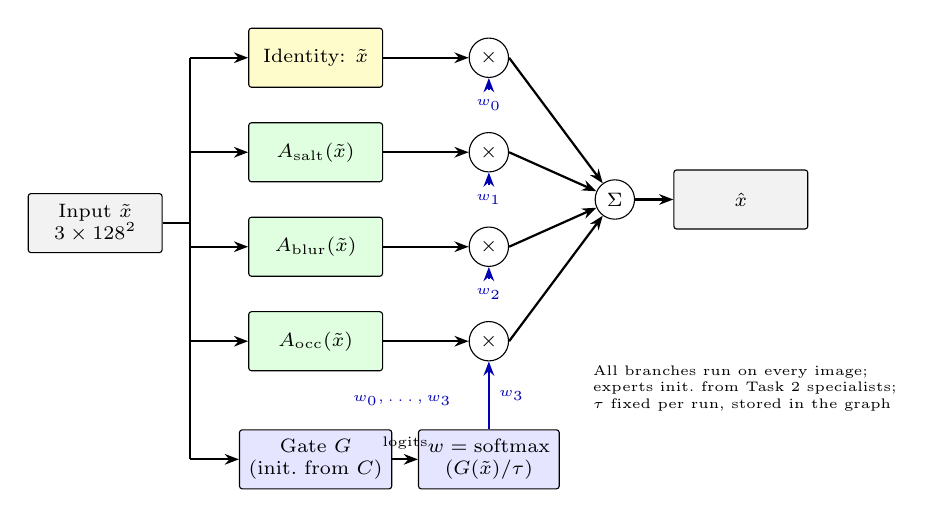
\begin{tikzpicture}[
    blk/.style={draw, rounded corners=1pt, minimum height=0.75cm, minimum width=1.7cm,
                align=center, font=\scriptsize},
    io/.style={blk, fill=gray!10},
    gate/.style={blk, fill=blue!10},
    exp/.style={blk, fill=green!12},
    idn/.style={blk, fill=yellow!20},
    op/.style={draw, circle, inner sep=1pt, minimum size=0.5cm, font=\scriptsize},
    arr/.style={-{Stealth[length=1.8mm]}, thick}
  ]
  \node[io]  (inp) at (0,0) {Input $\tilde{x}$\\$3\times128^2$};

  \node[idn] (b0) at (2.8,2.1)  {Identity: $\tilde{x}$};
  \node[exp] (b1) at (2.8,0.9)  {$A_{\mathrm{salt}}(\tilde{x})$};
  \node[exp] (b2) at (2.8,-0.3) {$A_{\mathrm{blur}}(\tilde{x})$};
  \node[exp] (b3) at (2.8,-1.5) {$A_{\mathrm{occ}}(\tilde{x})$};

  \node[op] (m0) at (5.0,2.1)  {$\times$};
  \node[op] (m1) at (5.0,0.9)  {$\times$};
  \node[op] (m2) at (5.0,-0.3) {$\times$};
  \node[op] (m3) at (5.0,-1.5) {$\times$};

  \node[op] (sum) at (6.6,0.3) {$\Sigma$};
  \node[io] (outp) at (8.2,0.3) {$\hat{x}$};

  \node[gate] (g)  at (2.8,-3.0) {Gate $G$\\(init.\ from $C$)};
  \node[gate] (sm) at (5.0,-3.0) {$w=\mathrm{softmax}$\\$(G(\tilde{x})/\tau)$};

  % Input to every branch and to the gate.
  \draw[thick] (inp.east) -- (1.2,0);
  \draw[thick] (1.2,2.1) -- (1.2,-3.0);
  \draw[arr] (1.2,2.1)  -- (b0.west);
  \draw[arr] (1.2,0.9)  -- (b1.west);
  \draw[arr] (1.2,-0.3) -- (b2.west);
  \draw[arr] (1.2,-1.5) -- (b3.west);
  \draw[arr] (1.2,-3.0) -- (g.west);

  \draw[arr] (b0) -- (m0);
  \draw[arr] (b1) -- (m1);
  \draw[arr] (b2) -- (m2);
  \draw[arr] (b3) -- (m3);

  \draw[arr] (g) -- node[above, font=\tiny] {logits} (sm);
  % Each multiplier receives its routing weight from below (blue labels);
  % the weights are the outputs of the softmax node.
  \node[font=\tiny, text=blue!70!black] (w0) at (5.0,1.5)  {$w_0$};
  \node[font=\tiny, text=blue!70!black] (w1) at (5.0,0.3)  {$w_1$};
  \node[font=\tiny, text=blue!70!black] (w2) at (5.0,-0.9) {$w_2$};
  \draw[arr, blue!70!black] (w0) -- (m0);
  \draw[arr, blue!70!black] (w1) -- (m1);
  \draw[arr, blue!70!black] (w2) -- (m2);
  \draw[arr, blue!70!black] (sm) -- node[right, font=\tiny] {$w_3$} (m3);
  \node[font=\tiny, text=blue!70!black, align=center] at (3.9,-2.25) {$w_0,\dots,w_3$};

  \draw[arr] (m0.east) -- (sum);
  \draw[arr] (m1.east) -- (sum);
  \draw[arr] (m2.east) -- (sum);
  \draw[arr] (m3.east) -- (sum);
  \draw[arr] (sum) -- (outp);

  \node[font=\tiny, align=left, anchor=west] at (6.2,-2.1)
    {All branches run on every image;\\experts init.\ from Task 2 specialists;\\$\tau$ fixed per run, stored in the graph};
\end{tikzpicture}%
}

\caption{Task~3 soft mixture-of-experts: every branch is evaluated and the
outputs are weighted by $w=\mathrm{softmax}(G(\tilde{x})/\tau)$.}
\label{fig:task3_arch}
\end{figure}

\subsection{Loss function}
The joint loss is
\begin{equation}
\begin{split}
\mathcal{L}_{\mathrm{MoE}} = {}& \lambda_1\mathcal{L}_1
 + \lambda_s(1-\mathrm{SSIM})\\
 &+ \lambda_c\mathcal{L}_{\mathrm{CE}}
 + \lambda_b\mathcal{L}_{\mathrm{balance}},\qquad \lambda_s = 1-\lambda_1,
\end{split}
\end{equation}
\begin{equation}
\mathcal{L}_{\mathrm{balance}} = \sum_{k=0}^{3}\left(\bar{w}_k-\tfrac14\right)^2,
\end{equation}
where $\bar{w}_k$ is the mean weight of branch $k$ over a batch. Because the
batches are exactly balanced (the Task~2 collate is reused), the ideal gate
gives $\bar{w}_k=\frac14$ and the balance term is zero; it grows when the gate
collapses onto a few branches. An entropy regulariser was considered; we kept
the squared form because it is the task's suggested term and is easy to
interpret. The cross-entropy is computed on $G(\tilde{x})/\tau$, i.e.\ on
exactly the distribution that produces the routing weights; on the raw
logits it would train the classifier but not the weights actually used for
mixing whenever $\tau\neq1$.

\subsection{Two-stage training}
In a warm-up stage the experts are frozen and only the gate is trained
(Adam, learning rate $5\times10^{-4}$). Freezing by disabling gradients alone
is insufficient: in training mode batch normalisation would still update its
running statistics, so the ``frozen'' experts would drift. The frozen experts
are therefore also kept in evaluation mode; tests confirm that they receive
no gradients and keep their batch-normalisation statistics. After the
warm-up all parameters are unfrozen and fine-tuned jointly with a smaller,
Optuna-selected learning rate and a cosine schedule. Batches contain 32
images (8 per class). The final run uses 3 warm-up and 25 fine-tuning
epochs; each epoch is validated on the balanced validation manifest with
Eq.~\eqref{eq:val_obj}, and the gate accuracy and mean branch weights are logged.

\subsection{Optuna search design}
Twenty trials of 2 warm-up and 6 fine-tuning epochs search the fine-tuning
learning rate, $\tau$, $\lambda_c$, $\lambda_b$ and $\lambda_1$
(Table~\ref{tab:task3_space}). Trial~0 is fixed to the suggested starting
point ($\lambda_1=0.8$, $\lambda_s=0.2$, $\lambda_c=0.1$, $\lambda_b=0.01$,
$\tau=1$, learning rate $10^{-4}$) as a reference. Trials are scored with
the same fixed objective as Tasks~1 and~2, which keeps the three tasks
comparable. In addition to the median pruner (five start-up trials, four
warm-up epochs), a trial is pruned for \emph{routing collapse} if, during
fine-tuning, the mean weight of any branch on the balanced validation set
falls below 0.05 (each branch would average 0.25 under perfect routing);
detecting collapse only after training would waste the trial's compute.

\begin{table}[t]
\centering
\caption{Task 3 Optuna search space and selected configuration.}
\label{tab:task3_space}
\footnotesize
\begin{tabular}{llc}
\toprule
Hyperparameter & Range (scale) & Selected \\
\midrule
Fine-tuning learning rate & $10^{-5}$--$3\times10^{-4}$ (log) & \na \\
Temperature $\tau$ & 0.5--3.0 (linear) & \na \\
CE weight $\lambda_c$ & 0.01--1 (log) & \na \\
Balance weight $\lambda_b$ & 0.001--0.1 (log) & \na \\
L1 weight $\lambda_1$ ($\lambda_s=1-\lambda_1$) & 0.5--0.95 (linear) & \na \\
\bottomrule
\end{tabular}
\\[3pt]
% TODO(results): fill from configs/task3_moe_best.yaml.
\TODO{Fill from \file{configs/task3_moe_best.yaml}.}
\end{table}

\subsection{Gate analysis protocol}
To check the gate objectively rather than by inspecting a few images, we
compute on the test manifest the mean of each branch weight per true
corruption and severity, the distribution of the weights per true
corruption, four examples where one expert dominates (highest maximum
weight, spread across corruptions) and four where the weight is shared
(highest routing entropy $-\sum_k w_k\log w_k$). A branch is called
\emph{inactive} if it is the top-weighted branch for fewer than 1\% of the
images and its mean weight is below 0.05, and \emph{dominating unrelated
inputs} if its mean weight on images of the other corruptions exceeds 0.5.
These thresholds are judgement calls, stated here so that they can be
challenged.

\subsection{Results}
% TODO(results): Task 3 Optuna outcome.
\TODO{Report completed trials, trials pruned by the median rule and for
routing collapse, the best trial and the selected $\tau$ and $\lambda$s
(Table~\ref{tab:optuna_summary}); describe how routing sharpness changed with $\tau$,
the curves across warm-up and fine-tuning (Fig.~\ref{fig:task3_curves}), and the
restoration results per condition and severity (Table~\ref{tab:task3_results}).}

\begin{figure}[t]
\centering
\figOrTodo{figures/task3_moe_curves.png}{\columnwidth}{Training loss terms, validation objective,
gate accuracy and mean branch weights per epoch across warm-up and fine-tuning (export from W\&B group task3-moe)}
\caption{Task 3 training and validation curves (the vertical line marks the end of the warm-up).}
\label{fig:task3_curves}
\end{figure}

\begin{table}[t]
\centering
\caption{Task 3 test results per condition and severity.}
\label{tab:task3_results}
\scriptsize
\setlength{\tabcolsep}{3pt}
\begin{tabular}{llrrrrr}
\toprule
Cond. & Sev. & In PSNR & PSNR & In SSIM & SSIM & L1 \\
\midrule
Clean & --   & \na & \na & \na & \na & \na \\
S\&P  & low  & \na & \na & \na & \na & \na \\
S\&P  & med. & \na & \na & \na & \na & \na \\
S\&P  & high & \na & \na & \na & \na & \na \\
Blur  & low  & \na & \na & \na & \na & \na \\
Blur  & med. & \na & \na & \na & \na & \na \\
Blur  & high & \na & \na & \na & \na & \na \\
Occl. & low  & \na & \na & \na & \na & \na \\
Occl. & med. & \na & \na & \na & \na & \na \\
Occl. & high & \na & \na & \na & \na & \na \\
\midrule
Corr. & all & \na & \na & \na & \na & \na \\
All       & all & \na & \na & \na & \na & \na \\
\bottomrule
\end{tabular}
\\[3pt]
% TODO(results): fill from report/results/task3_moe_test_metrics.csv.
\TODO{Fill from \file{report/results/task3_moe_test_metrics.csv}.}
\end{table}

\begin{table}[t]
\centering
\caption{Mean routing weight per true corruption and severity (test set).
Ideal routing puts a weight near 1 on the matching branch.}
\label{tab:task3_weights}
\scriptsize
\setlength{\tabcolsep}{4pt}
\begin{tabular}{llcccc}
\toprule
Cond. & Sev. & $w_0$ (id.) & $w_1$ (S\&P) & $w_2$ (blur) & $w_3$ (occl.) \\
\midrule
Clean & --   & \na & \na & \na & \na \\
S\&P  & low  & \na & \na & \na & \na \\
S\&P  & med. & \na & \na & \na & \na \\
S\&P  & high & \na & \na & \na & \na \\
Blur  & low  & \na & \na & \na & \na \\
Blur  & med. & \na & \na & \na & \na \\
Blur  & high & \na & \na & \na & \na \\
Occl. & low  & \na & \na & \na & \na \\
Occl. & med. & \na & \na & \na & \na \\
Occl. & high & \na & \na & \na & \na \\
\bottomrule
\end{tabular}
\\[3pt]
% TODO(results): fill from report/results/task3_moe_mean_weights.csv.
\TODO{Fill from \file{report/results/task3_moe_mean_weights.csv}.}
\end{table}

\begin{figure}[t]
\centering
\figOrTodo{figures/task3_moe_routing_heatmap.png}{\columnwidth}{Routing heatmap: mean weight per (true corruption, severity) and branch}
\caption{Task 3 routing heatmap on the test manifest.}
\label{fig:task3_heatmap}
\end{figure}

\begin{figure}[t]
\centering
\figOrTodo{figures/task3_moe_weight_distribution.png}{\columnwidth}{Box plots of the four branch weights per true corruption}
\caption{Task 3 distribution of the routing weights per true corruption.}
\label{fig:task3_distribution}
\end{figure}

\begin{table}[t]
\centering
\caption{Expert health on the test set (criteria in Section~\ref{sec:task3}).}
\label{tab:task3_health}
\footnotesize
\begin{tabular}{lccc}
\toprule
Branch & Top-1 (\%) & Mean $w$ & Mean $w$ (other corr.) \\
\midrule
Identity        & \na & \na & \na \\
Salt-and-pepper & \na & \na & \na \\
Blur            & \na & \na & \na \\
Occlusion       & \na & \na & \na \\
\bottomrule
\end{tabular}
\\[3pt]
% TODO(results): fill from report/results/task3_moe_expert_health.csv; state inactive / dominating branches (or "none").
\TODO{Fill from \file{report/results/task3_moe_expert_health.csv}; state
which branches (if any) are inactive or dominate unrelated inputs.}
\end{table}

% TODO(results): interpret routing tables/figures.
\TODO{Interpret Tables~\ref{tab:task3_weights}--\ref{tab:task3_health} and
Figs.~\ref{fig:task3_heatmap}--\ref{fig:task3_distribution}: how sharply the
gate routes each corruption, how this changes with severity, and whether any
expert is inactive or dominating.}

\begin{figure*}[t]
\centering
\begin{minipage}{0.49\textwidth}\centering
\figOrTodo{figures/task3_moe_dominant_examples.png}{\linewidth}{Four examples in which one expert dominates}
\end{minipage}\hfill
\begin{minipage}{0.49\textwidth}\centering
\figOrTodo{figures/task3_moe_distributed_examples.png}{\linewidth}{Four examples with weight shared across experts (highest routing entropy)}
\end{minipage}
\caption{Task 3 routing examples. Left: one expert dominates. Right: weight
shared across several branches. Row labels give the four weights.}
\label{fig:task3_examples}
\end{figure*}

% TODO(results): discuss dominant vs distributed examples.
\TODO{Discuss Fig.~\ref{fig:task3_examples}: what kinds of inputs receive
shared weights, and whether mixing helps or hurts them.}

\subsection{Comparison with Tasks 1 and 2}
\begin{table}[t]
\centering
\caption{Restoration systems compared on the corrupted test items (33,021
items; clean inputs excluded) and on clean inputs.}
\label{tab:compare}
\scriptsize
\setlength{\tabcolsep}{4pt}
\begin{tabular}{lcccc}
\toprule
 & \multicolumn{2}{c}{Corrupted} & \multicolumn{2}{c}{Clean} \\
\cmidrule(lr){2-3}\cmidrule(lr){4-5}
System & PSNR & SSIM & PSNR & SSIM \\
\midrule
Input (no restoration)        & \na & \na & --  & --  \\
Task 1 universal AE           & \na & \na & \na & \na \\
Task 2 oracle routing         & \na & \na & \na & \na \\
Task 2 predicted routing      & \na & \na & \na & \na \\
Task 3 soft MoE               & \na & \na & \na & \na \\
\bottomrule
\end{tabular}
\\[3pt]
% TODO(results): "corrupted / all" and "clean" rows of the Task 1, 2 and 3 result CSVs.
\TODO{Fill from the ``corrupted/all'' and ``clean'' rows of the Task 1--3 CSVs.}
\end{table}

% TODO(results): interpret the comparison.
\TODO{Interpret Table~\ref{tab:compare}: does soft routing recover the
misrouting losses of Task~2, and how do both compare with the universal model?}

\subsection{Failure cases}
\begin{figure*}[t]
\centering
\figOrTodo{figures/task3_moe_failures.png}{0.85\textwidth}{Four failure cases (lowest SSIM per condition) with routing weights}
\caption{Task 3 failure cases (lowest SSIM per condition), labelled with the routing weights.}
\label{fig:task3_failures}
\end{figure*}
% TODO(results): discuss the Task 3 failures.
\TODO{Explain the failures in Fig.~\ref{fig:task3_failures}; distinguish
routing errors from expert errors using the weights in the row labels.
Representative examples are in \file{figures/task3_moe_examples.png}.}

\subsection{Discussion}
% TODO(results): Task 3 discussion.
\TODO{Discuss what the gate learned during joint training compared with
the initial classifier, the effect of $\tau$ and the balance term, and the
computational cost of evaluating all experts.}

% =====================================================================
\section{Task 4: Style-Conditioned Face-to-Sketch GAN}
\label{sec:task4}

\subsection{Architecture and style conditioning}
The generator $\hat{y}=G(x,s)$ (Fig.~\ref{fig:task4_arch}) follows the
pix2pix U-Net~\cite{isola2017image,ronneberger2015unet} adapted to
$128\times128$: seven stride-2 $4\times4$ convolutions reduce the input to
$1\times1$ ($c, 2c, 4c, 8c, 8c, 8c, 8c$ channels, LeakyReLU 0.2), and seven
stride-2 transposed convolutions restore it, with skip connections from each
encoder level to the matching decoder level, dropout in the three innermost
decoder layers and a $\tanh$ output. Batch normalisation is used everywhere
except in the first encoder layer and at the $1\times1$ bottleneck, where it
would be undefined at batch size 1. Weights are initialised from
$\mathcal{N}(0,0.02)$. Unlike Task~1, the generator keeps pix2pix's
transposed convolutions; we did not investigate an upsample-and-convolve
decoder for Task~4.

The discriminator $D(x,y,s)$ is a $70\times70$ PatchGAN
(C64--C128--C256--C512 followed by a one-channel convolution); for a
$128\times128$ input it outputs a $14\times14$ map of real/fake logits, each
of which sees a $70\times70$ patch of the photo--sketch pair.

The style $s\in\{1,2,3\}$ is represented by a learned categorical embedding
(\texttt{nn.Embedding}) of size $d_s$, and each network has its \emph{own}
embedding: sharing one would couple the parameters of the two adversaries.
The generator receives the style twice: as a broadcast $d_s$-channel map
concatenated with the photo at the input, so the early layers that form
strokes and texture can depend on it, and concatenated with the $1\times1$
bottleneck, so the decoder has direct access to it where the global
decision is made. The discriminator receives the style as a broadcast map
concatenated with the photo and the real or generated sketch. One-hot style
channels (not a learned embedding), injection at the input only, and
feature-wise modulation in every layer were considered; the latter is more
expressive but not required. Tests confirm that changing $s$ changes both
the generated sketch and the discriminator logits and that gradients reach
both embeddings. With $d_s=16$ the generator has 10,535,571 / 41,977,075
parameters and the discriminator 704,465 / 2,785,137 at base width 32 / 64.

\begin{figure}[t]
\centering
% Task 4: style-conditioned U-Net generator and PatchGAN discriminator
% (src/models/cgan.py). c = base channels, d_s = style embedding size.
% Included from main.tex with % Task 4: style-conditioned U-Net generator and PatchGAN discriminator
% (src/models/cgan.py). c = base channels, d_s = style embedding size.
% Included from main.tex with % Task 4: style-conditioned U-Net generator and PatchGAN discriminator
% (src/models/cgan.py). c = base channels, d_s = style embedding size.
% Included from main.tex with \input{figures/tikz/task4_cgan}.
\resizebox{\columnwidth}{!}{%
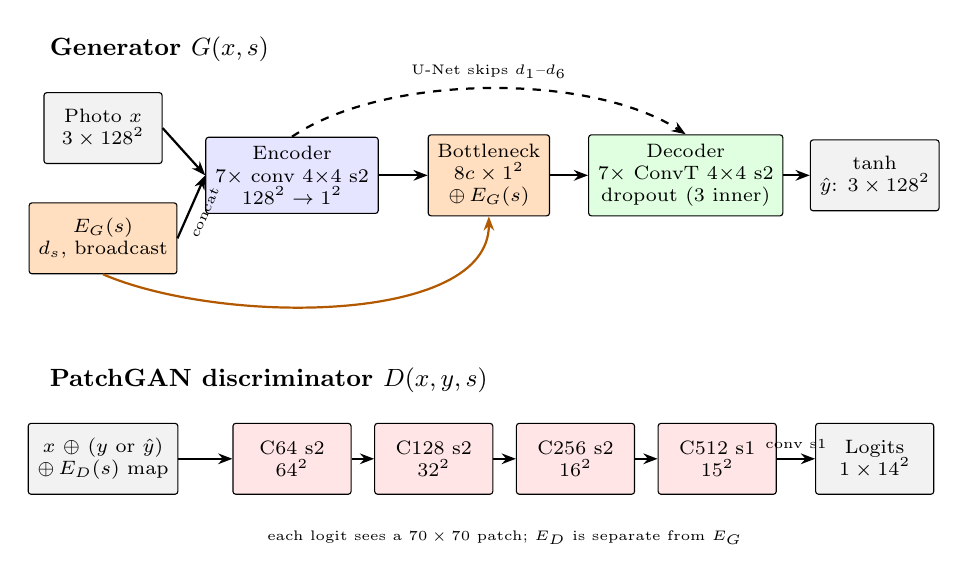
\begin{tikzpicture}[
    blk/.style={draw, rounded corners=1pt, minimum height=0.9cm, minimum width=1.5cm,
                align=center, font=\scriptsize},
    io/.style={blk, fill=gray!10},
    emb/.style={blk, fill=orange!25},
    enc/.style={blk, fill=blue!10},
    dec/.style={blk, fill=green!12},
    dis/.style={blk, fill=red!10},
    arr/.style={-{Stealth[length=1.8mm]}, thick}
  ]
  % ---------------- Generator ----------------
  \node[font=\small\bfseries, anchor=west] at (-0.8,1.6) {Generator $G(x,s)$};
  \node[io]  (x)   at (0,0.6)   {Photo $x$\\$3\times128^2$};
  \node[emb] (eg)  at (0,-0.8)  {$E_G(s)$\\$d_s$, broadcast};
  \node[enc] (gen) at (2.4,0)   {Encoder\\7$\times$ conv $4{\times}4$ s2\\$128^2\rightarrow1^2$};
  \node[emb] (bn)  at (4.9,0)   {Bottleneck\\$8c\times1^2$\\$\oplus\,E_G(s)$};
  \node[dec] (gde) at (7.4,0)   {Decoder\\7$\times$ ConvT $4{\times}4$ s2\\dropout (3 inner)};
  \node[io]  (yh)  at (9.8,0)   {$\tanh$\\$\hat{y}$: $3\times128^2$};

  \draw[arr] (x.east) -- (gen.west);
  \draw[arr] (eg.east) -- node[below, font=\tiny, sloped] {concat} (gen.west);
  \draw[arr] (gen) -- (bn);
  \draw[arr] (bn) -- (gde);
  \draw[arr] (gde) -- (yh);
  \draw[arr, dashed] (gen.north) .. controls (3.6,1.3) and (6.2,1.3) .. node[above, font=\tiny] {U-Net skips $d_1$--$d_6$} (gde.north);
  \draw[arr, orange!70!black] (eg.south) .. controls (1.5,-1.9) and (4.9,-1.9) .. (bn.south);

  % ---------------- Discriminator ----------------
  \node[font=\small\bfseries, anchor=west] at (-0.8,-2.6) {PatchGAN discriminator $D(x,y,s)$};
  \node[io]  (dx)  at (0,-3.6)  {$x$ $\oplus$ ($y$ or $\hat{y}$)\\$\oplus\,E_D(s)$ map};
  \node[dis] (c1)  at (2.4,-3.6) {C64 s2\\$64^2$};
  \node[dis] (c2)  at (4.2,-3.6) {C128 s2\\$32^2$};
  \node[dis] (c3)  at (6.0,-3.6) {C256 s2\\$16^2$};
  \node[dis] (c4)  at (7.8,-3.6) {C512 s1\\$15^2$};
  \node[io]  (lg)  at (9.8,-3.6) {Logits\\$1\times14^2$};
  \draw[arr] (dx) -- (c1);
  \draw[arr] (c1) -- (c2);
  \draw[arr] (c2) -- (c3);
  \draw[arr] (c3) -- (c4);
  \draw[arr] (c4) -- node[above, font=\tiny] {conv s1} (lg);
  \node[font=\tiny, align=center] at (5.1,-4.6)
    {each logit sees a $70\times70$ patch; $E_D$ is separate from $E_G$};
\end{tikzpicture}%
}
.
\resizebox{\columnwidth}{!}{%
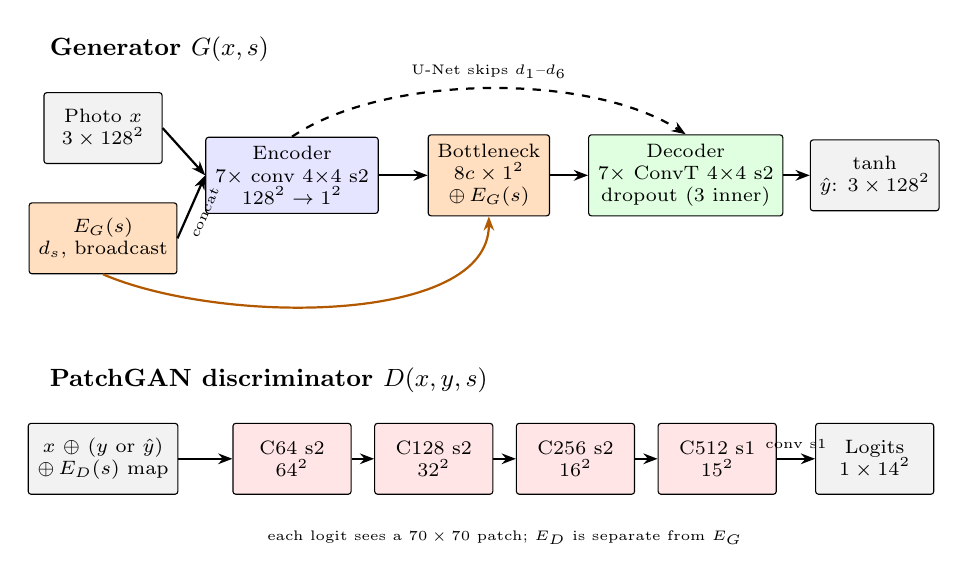
\begin{tikzpicture}[
    blk/.style={draw, rounded corners=1pt, minimum height=0.9cm, minimum width=1.5cm,
                align=center, font=\scriptsize},
    io/.style={blk, fill=gray!10},
    emb/.style={blk, fill=orange!25},
    enc/.style={blk, fill=blue!10},
    dec/.style={blk, fill=green!12},
    dis/.style={blk, fill=red!10},
    arr/.style={-{Stealth[length=1.8mm]}, thick}
  ]
  % ---------------- Generator ----------------
  \node[font=\small\bfseries, anchor=west] at (-0.8,1.6) {Generator $G(x,s)$};
  \node[io]  (x)   at (0,0.6)   {Photo $x$\\$3\times128^2$};
  \node[emb] (eg)  at (0,-0.8)  {$E_G(s)$\\$d_s$, broadcast};
  \node[enc] (gen) at (2.4,0)   {Encoder\\7$\times$ conv $4{\times}4$ s2\\$128^2\rightarrow1^2$};
  \node[emb] (bn)  at (4.9,0)   {Bottleneck\\$8c\times1^2$\\$\oplus\,E_G(s)$};
  \node[dec] (gde) at (7.4,0)   {Decoder\\7$\times$ ConvT $4{\times}4$ s2\\dropout (3 inner)};
  \node[io]  (yh)  at (9.8,0)   {$\tanh$\\$\hat{y}$: $3\times128^2$};

  \draw[arr] (x.east) -- (gen.west);
  \draw[arr] (eg.east) -- node[below, font=\tiny, sloped] {concat} (gen.west);
  \draw[arr] (gen) -- (bn);
  \draw[arr] (bn) -- (gde);
  \draw[arr] (gde) -- (yh);
  \draw[arr, dashed] (gen.north) .. controls (3.6,1.3) and (6.2,1.3) .. node[above, font=\tiny] {U-Net skips $d_1$--$d_6$} (gde.north);
  \draw[arr, orange!70!black] (eg.south) .. controls (1.5,-1.9) and (4.9,-1.9) .. (bn.south);

  % ---------------- Discriminator ----------------
  \node[font=\small\bfseries, anchor=west] at (-0.8,-2.6) {PatchGAN discriminator $D(x,y,s)$};
  \node[io]  (dx)  at (0,-3.6)  {$x$ $\oplus$ ($y$ or $\hat{y}$)\\$\oplus\,E_D(s)$ map};
  \node[dis] (c1)  at (2.4,-3.6) {C64 s2\\$64^2$};
  \node[dis] (c2)  at (4.2,-3.6) {C128 s2\\$32^2$};
  \node[dis] (c3)  at (6.0,-3.6) {C256 s2\\$16^2$};
  \node[dis] (c4)  at (7.8,-3.6) {C512 s1\\$15^2$};
  \node[io]  (lg)  at (9.8,-3.6) {Logits\\$1\times14^2$};
  \draw[arr] (dx) -- (c1);
  \draw[arr] (c1) -- (c2);
  \draw[arr] (c2) -- (c3);
  \draw[arr] (c3) -- (c4);
  \draw[arr] (c4) -- node[above, font=\tiny] {conv s1} (lg);
  \node[font=\tiny, align=center] at (5.1,-4.6)
    {each logit sees a $70\times70$ patch; $E_D$ is separate from $E_G$};
\end{tikzpicture}%
}
.
\resizebox{\columnwidth}{!}{%
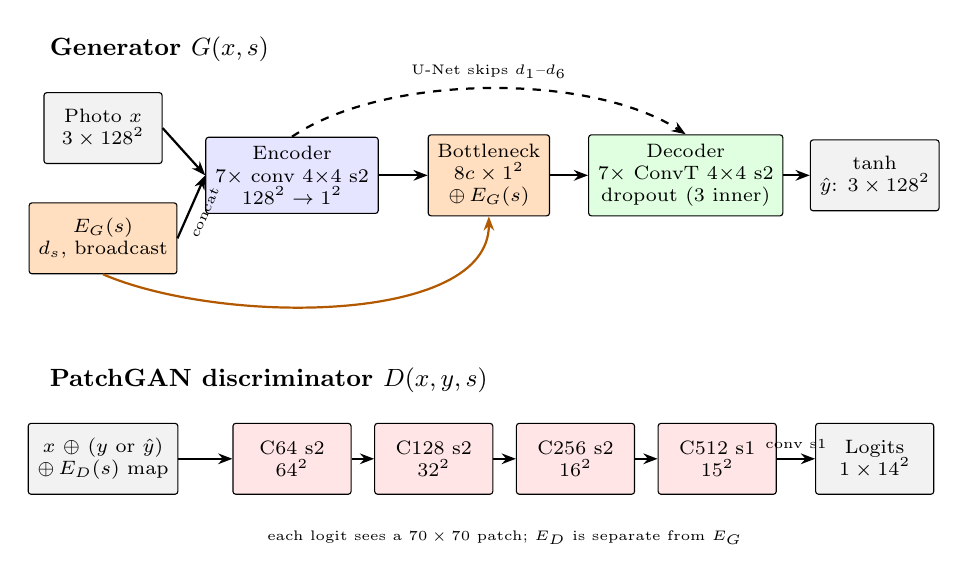
\begin{tikzpicture}[
    blk/.style={draw, rounded corners=1pt, minimum height=0.9cm, minimum width=1.5cm,
                align=center, font=\scriptsize},
    io/.style={blk, fill=gray!10},
    emb/.style={blk, fill=orange!25},
    enc/.style={blk, fill=blue!10},
    dec/.style={blk, fill=green!12},
    dis/.style={blk, fill=red!10},
    arr/.style={-{Stealth[length=1.8mm]}, thick}
  ]
  % ---------------- Generator ----------------
  \node[font=\small\bfseries, anchor=west] at (-0.8,1.6) {Generator $G(x,s)$};
  \node[io]  (x)   at (0,0.6)   {Photo $x$\\$3\times128^2$};
  \node[emb] (eg)  at (0,-0.8)  {$E_G(s)$\\$d_s$, broadcast};
  \node[enc] (gen) at (2.4,0)   {Encoder\\7$\times$ conv $4{\times}4$ s2\\$128^2\rightarrow1^2$};
  \node[emb] (bn)  at (4.9,0)   {Bottleneck\\$8c\times1^2$\\$\oplus\,E_G(s)$};
  \node[dec] (gde) at (7.4,0)   {Decoder\\7$\times$ ConvT $4{\times}4$ s2\\dropout (3 inner)};
  \node[io]  (yh)  at (9.8,0)   {$\tanh$\\$\hat{y}$: $3\times128^2$};

  \draw[arr] (x.east) -- (gen.west);
  \draw[arr] (eg.east) -- node[below, font=\tiny, sloped] {concat} (gen.west);
  \draw[arr] (gen) -- (bn);
  \draw[arr] (bn) -- (gde);
  \draw[arr] (gde) -- (yh);
  \draw[arr, dashed] (gen.north) .. controls (3.6,1.3) and (6.2,1.3) .. node[above, font=\tiny] {U-Net skips $d_1$--$d_6$} (gde.north);
  \draw[arr, orange!70!black] (eg.south) .. controls (1.5,-1.9) and (4.9,-1.9) .. (bn.south);

  % ---------------- Discriminator ----------------
  \node[font=\small\bfseries, anchor=west] at (-0.8,-2.6) {PatchGAN discriminator $D(x,y,s)$};
  \node[io]  (dx)  at (0,-3.6)  {$x$ $\oplus$ ($y$ or $\hat{y}$)\\$\oplus\,E_D(s)$ map};
  \node[dis] (c1)  at (2.4,-3.6) {C64 s2\\$64^2$};
  \node[dis] (c2)  at (4.2,-3.6) {C128 s2\\$32^2$};
  \node[dis] (c3)  at (6.0,-3.6) {C256 s2\\$16^2$};
  \node[dis] (c4)  at (7.8,-3.6) {C512 s1\\$15^2$};
  \node[io]  (lg)  at (9.8,-3.6) {Logits\\$1\times14^2$};
  \draw[arr] (dx) -- (c1);
  \draw[arr] (c1) -- (c2);
  \draw[arr] (c2) -- (c3);
  \draw[arr] (c3) -- (c4);
  \draw[arr] (c4) -- node[above, font=\tiny] {conv s1} (lg);
  \node[font=\tiny, align=center] at (5.1,-4.6)
    {each logit sees a $70\times70$ patch; $E_D$ is separate from $E_G$};
\end{tikzpicture}%
}

\caption{Task~4 networks. Top: U-Net generator with the style embedding
$E_G(s)$ at the input and at the bottleneck. Bottom: PatchGAN discriminator
with its own embedding $E_D(s)$.}
\label{fig:task4_arch}
\end{figure}

\subsection{Loss functions}
With binary cross-entropy on logits,
\begin{align}
\mathcal{L}_D &= \tfrac12\bigl[\mathrm{BCE}(D(x,y,s),1)
  + \mathrm{BCE}(D(x,G(x,s),s),0)\bigr],\\
\mathcal{L}_G &= \mathrm{BCE}(D(x,G(x,s),s),1)
  + \lambda_{L1}\,\lVert y-G(x,s)\rVert_1 .
\end{align}
The discriminator loss is halved as in pix2pix~\cite{isola2017image}.
Photographs and sketches are scaled to $[-1,1]$ during training; the export
wrapper maps the application's $[0,1]$ input and output to and from this
range.

\subsection{Training procedure and logging}
Each iteration first updates $D$ on a real and a generated (detached) pair,
then updates $G$. Both use Adam with $\beta=(0.5,0.999)$ and constant
learning rates; the final configuration is trained for 200 epochs with the
paired augmentation of Section~\ref{sec:data}. The discriminator real loss,
discriminator fake loss, generator adversarial loss and generator L1 loss
are logged separately every epoch, together with the validation L1, PSNR and
SSIM (overall and per style). At epoch 1 and every 10 epochs the same
validation photographs (two per style) are logged as a grid showing the
photo, the true sketch, the generated sketch and the same photo in all three
styles, so that the generator's development can be followed over time.

\subsection{Optuna search design and model selection}
GAN losses oscillate by design and do not track output quality, so they
cannot be used for selection. FID~\cite{heusel2017gans} is the standard
measure of GAN output, but it compares feature statistics of two image sets,
and with about 160 validation images the estimate would be strongly biased
and noisy; it also requires an Inception network.
% TODO: confirm the sample-size statement against Heusel et al. before submission.
Because FS2K is paired, we instead score every trial and epoch against the
ground-truth sketches with
\begin{equation}
J_{\mathrm{GAN}} = 0.5\,\mathcal{L}_1 + 0.5\,(1-\mathrm{SSIM})
\end{equation}
on images in $[0,1]$, with the generator in evaluation mode (dropout off).
This rewards correct structure but may favour slightly smoother sketches;
we return to this in Section~\ref{sec:limitations}. Twelve trials of 25
epochs are run (TPE, median pruner with four start-up trials and ten warm-up
epochs); trial~0 is fixed to the pix2pix-style defaults (learning rates
$2\times10^{-4}$, batch size 4, $c=64$, dropout 0.5, $d_s=16$,
$\lambda_{L1}=100$). The best configuration is then retrained for the full
200 epochs. Table~\ref{tab:task4_space} gives the search space.

\begin{table}[t]
\centering
\caption{Task 4 Optuna search space and selected configuration.}
\label{tab:task4_space}
\footnotesize
\begin{tabular}{llc}
\toprule
Hyperparameter & Range (scale) & Selected \\
\midrule
Generator learning rate & $5\times10^{-5}$--$5\times10^{-4}$ (log) & \na \\
Discriminator learning rate & $5\times10^{-5}$--$5\times10^{-4}$ (log) & \na \\
Batch size & \{1, 4, 8, 16\} & \na \\
Base channels $c$ & \{32, 48, 64\} & \na \\
Dropout (generator) & 0--0.5 (linear) & \na \\
Style embedding size $d_s$ & \{8, 16, 32\} & \na \\
$\lambda_{L1}$ & 10--200 (log) & \na \\
\bottomrule
\end{tabular}
\\[3pt]
% TODO(results): fill from configs/task4_cgan_best.yaml.
\TODO{Fill from \file{configs/task4_cgan_best.yaml}.}
\end{table}

\subsection{Results}
% TODO(results): Task 4 Optuna outcome.
\TODO{Report completed/pruned trials, best trial and selected configuration
(Table~\ref{tab:optuna_summary}); comment on the selected $\lambda_{L1}$
relative to the pix2pix default of 100.}

\begin{figure}[t]
\centering
\figOrTodo{figures/task4_cgan_curves.png}{\columnwidth}{D real, D fake, G adversarial and G L1 losses and
validation SSIM/objective per epoch of the final 200-epoch run (export from W\&B group task4-cgan)}
\caption{Task 4 training losses and validation measurements.}
\label{fig:task4_curves}
\end{figure}

\begin{figure}[t]
\centering
\figOrTodo{figures/task4_cgan_progress.png}{\columnwidth}{Fixed validation samples logged at several epochs (e.g.\ 1, 50, 100, 200), taken from the W\&B ``samples'' panel}
\caption{Task 4 generator development on fixed validation photographs.}
\label{fig:task4_progress}
\end{figure}

% TODO(results): interpret the GAN curves and progress grid.
\TODO{Interpret Figs.~\ref{fig:task4_curves}--\ref{fig:task4_progress}:
balance between $D$ and $G$, signs of instability or mode collapse, and
when the validation objective stopped improving.}

\begin{table}[t]
\centering
\caption{Task 4 results on the official FS2K test split.}
\label{tab:task4_results}
\footnotesize
\begin{tabular}{lrccc}
\toprule
Group & Count & L1 & PSNR & SSIM \\
\midrule
All     & \na & \na & \na & \na \\
Style 1 & \na & \na & \na & \na \\
Style 2 & \na & \na & \na & \na \\
Style 3 & \na & \na & \na & \na \\
\bottomrule
\end{tabular}
\\[3pt]
% TODO(results): fill from report/results/task4_cgan_test_metrics.csv.
\TODO{Fill from \file{report/results/task4_cgan_test_metrics.csv}.}
\end{table}

\begin{figure}[t]
\centering
\figOrTodo{figures/task4_cgan_examples.png}{\columnwidth}{Test photo, true sketch and generated sketch, three examples per style}
\caption{Task 4 test examples (photo, true sketch, generated sketch).}
\label{fig:task4_examples}
\end{figure}

\begin{figure}[t]
\centering
\figOrTodo{figures/task4_cgan_style_swap.png}{\columnwidth}{Five test photos rendered in all three styles}
\caption{Task 4 style swap: the same photograph generated in Styles 1--3.}
\label{fig:task4_swap}
\end{figure}

% TODO(results): interpret Task 4 table and figures.
\TODO{Interpret Table~\ref{tab:task4_results} and
Figs.~\ref{fig:task4_examples}--\ref{fig:task4_swap}: per-style quality and
whether the style condition visibly changes the output.}

\subsection{Failure cases}
\begin{figure}[t]
\centering
\figOrTodo{figures/task4_cgan_failures.png}{\columnwidth}{The four test pairs with the lowest SSIM}
\caption{Task 4 failure cases (lowest test SSIM).}
\label{fig:task4_failures}
\end{figure}
% TODO(results): discuss the four Task 4 failures.
\TODO{Explain the four failures of Fig.~\ref{fig:task4_failures} (e.g.\
unusual pose, lighting, accessories or background).}

\subsection{Discussion}
% TODO(results): Task 4 discussion.
\TODO{Discuss the trade-off between the adversarial and L1 terms, and how
well a paired L1/SSIM selection criterion agreed with visual quality.}

% =====================================================================
\section{Experimental Setup and Reproducibility}
\label{sec:setup}

\subsection{Hardware and software}
The development machine has only integrated graphics (Intel Iris Xe, no CUDA
device, 15.75\,GB RAM), so it runs a CPU-only PyTorch build
(\texttt{torch 2.14.1+cpu}) for development, unit tests and inference. All
training runs in Kaggle GPU notebooks, which clone the repository and call
the same command-line scripts; Google Colab was kept as a fallback.
% TODO(results): Kaggle GPU model, session limits, and epoch timings.
\TODO{State the Kaggle GPU model and, if measured, the time per epoch on the
laptop CPU vs.\ the Kaggle GPU for the same configuration.}

\subsection{Experiment tracking and Optuna}
Every Optuna trial, final training run and evaluation is a W\&B run in the
project \texttt{genai-a1}, grouped by task (e.g.\ \texttt{task1-udae}) and
named \texttt{trial-NNN}, \texttt{final-<model>} or \texttt{eval-<model>};
final checkpoints are uploaded as W\&B model artifacts. We chose W\&B over a
local MLflow file store because Kaggle sessions are wiped at the end, while
W\&B keeps the runs online. All studies use the TPE sampler with seed 42 and
are stored in SQLite (\file{optuna_studies/<study>.db}), so an interrupted
search can be resumed and the studies can be inspected later; the best
parameters are written to \file{configs/<task>_best.yaml}, which the final
training reads. Table~\ref{tab:optuna_summary} summarises the studies.
% TODO: add the public W&B project link.
\TODO{Add the W\&B project link.}

\begin{table}[t]
\centering
\caption{Optuna studies: design and outcome.}
\label{tab:optuna_summary}
\scriptsize
\setlength{\tabcolsep}{3pt}
\begin{tabular}{lccccc}
\toprule
Study & Trials$\times$ep. & Compl. & Pruned & Best & Best value \\
\midrule
Task 1 UDAE & 30$\times$10 & \na & \na & \na & \na \\
Task 2 classifier & 25$\times$8  & \na & \na & \na & \na \\
Task 2 specialists & 20$\times$8  & \na & \na & \na & \na \\
Task 3 MoE & 20$\times$(2+6) & \na & \na & \na & \na \\
Task 4 cGAN & 12$\times$25 & \na & \na & \na & \na \\
\bottomrule
\end{tabular}
\\[3pt]
% TODO(results): counts from the training logs / optuna_studies/*.db; for task3 also the number pruned for routing collapse.
\TODO{Fill from the Optuna studies; objectives: Tasks 1--3 minimise $J$
(Eq.~\eqref{eq:val_obj}), the classifier maximises macro-F1, Task~4 minimises
$J_{\mathrm{GAN}}$.}
\end{table}

\subsection{Reproducibility}
Python, NumPy and PyTorch are seeded with 42 before every run, cuDNN is set
to deterministic algorithms, data-loader shuffling uses a seeded generator,
and worker processes are seeded from PyTorch's per-worker seed. The Pet
split, the FS2K split and both corruption manifests are committed files.
The data, model, routing, mixture and GAN code is covered by unit tests
(pytest); end-to-end smoke runs on CPU with a few batches exercised every
script before the Kaggle runs. These smoke runs used untrained models and
their outputs were discarded; they are not results.

\subsection{ONNX export and verification}
All seven inference models are exported with ONNX opset 17 using
PyTorch's TorchScript-based exporter and a dynamic batch dimension: the
Task~1 autoencoder, the Task~2 classifier and three specialists as four
separate files, the complete Task~3 pipeline (gate, $\tau$, experts and
mixing) as one graph that returns the image, the weights and the logits,
and the Task~4 generator wrapped to accept and return $[0,1]$ images and an
integer style. Each export is run with ONNX Runtime on the same inputs as
PyTorch (the first 16 validation-manifest items, covering all four
conditions, for Tasks~1--3; six random images, two per style, for Task~4),
and the export fails if the maximum absolute
difference exceeds $10^{-4}$. Table~\ref{tab:onnx} will list the measured
differences.

\begin{table}[t]
\centering
\caption{Maximum absolute PyTorch--ONNX difference of the trained models
(tolerance $10^{-4}$).}
\label{tab:onnx}
\footnotesize
\begin{tabular}{lc}
\toprule
Model & Max.\ abs.\ difference \\
\midrule
\texttt{task1\_udae}                   & \na \\
\texttt{task2\_classifier}             & \na \\
\texttt{task2\_specialist\_salt\_pepper} & \na \\
\texttt{task2\_specialist\_blur}       & \na \\
\texttt{task2\_specialist\_occlusion}  & \na \\
\texttt{task3\_moe} (image / weights)  & \na \\
\texttt{task4\_generator}              & \na \\
\bottomrule
\end{tabular}
\\[3pt]
% TODO(results): fill from report/results/*_onnx_check.json.
\TODO{Fill from \file{report/results/*_onnx_check.json}.}
\end{table}

\subsection{Engineering difficulties and how they were resolved}
\begin{itemize}
  \item \emph{Blocked library files on the development machine.} Windows
  Smart App Control blocked compiled extension files in the virtual
  environment, which broke SQLAlchemy and hence Optuna's SQLite storage.
  Rather than disabling the security feature, SQLAlchemy was reinstalled
  without compiled extensions; the Optuna storage tests then passed. This
  affects only the laptop; Kaggle and the containers run Linux.
  \item \emph{Blurred values above 1.} The first run on the real data showed
  blurred pixel values slightly above 1.0 from floating-point rounding; the
  blur output is now clamped to $[0,1]$.
  \item \emph{Inflated averages.} The Task~2 smoke run showed that clean
  images returned unchanged score the capped 100\,dB and dominate overall
  means; the ``corrupted'' summary row and the SSIM-loss column for
  misrouted images were added in response.
  \item \emph{Frozen experts drifting.} A gradient-only freeze would still
  update batch-normalisation statistics during the Task~3 warm-up; the
  frozen experts are therefore held in evaluation mode.
  \item \emph{Redundant validation pass.} Task~3 validation initially passed
  over the data twice (once for images, once for weights); it now records
  the weights in the same pass.
  \item \emph{Model distribution.} Git LFS was rejected because of its free
  storage and bandwidth quota (Section~\ref{sec:app}).
\end{itemize}

% =====================================================================
\section{Application}
\label{sec:app}

\subsection{Design in Google Stitch}
The visual design, page structure, colours, controls, cards, image panels
and responsive layout were first developed in Google Stitch as a project
named \emph{RestoreLab}: a neutral light interface with white cards, one
accent colour and a fixed colour per input condition, with one screen per
workspace plus loading and error states. The prompts are kept in
\file{docs/stitch_prompts.md}.
% TODO: Stitch evidence (screenshots + prompt-and-screen screenshot with date) in report/figures/stitch/.
\TODO{Insert the Stitch evidence (Fig.~\ref{fig:stitch}) and state which
prompts were actually used and what was changed between the Stitch design
and the implementation.}

\begin{figure*}[t]
\centering
\begin{minipage}{0.49\textwidth}\centering
\figOrTodo{figures/stitch/stitch_project_canvas.png}{\linewidth}{Stitch project canvas showing all generated screens}
\end{minipage}\hfill
\begin{minipage}{0.49\textwidth}\centering
\figOrTodo{figures/stitch/02_universal_restoration.png}{\linewidth}{Stitch screen of a workspace, ideally with the prompt visible and dated}
\end{minipage}
\caption{Evidence of the original Google Stitch design. Left: the project
canvas. Right: a generated workspace screen.}
\label{fig:stitch}
\end{figure*}

\subsection{Architecture}
Fig.~\ref{fig:app_arch} shows the deployed system. Two Docker containers are
started by a single \texttt{docker compose up --build}: the \emph{frontend}
container runs nginx, which serves the built React application and forwards
every \texttt{/api/} request to the \emph{backend} container, which runs
FastAPI with ONNX Runtime and no PyTorch. The ONNX files and the sample
images are mounted read-only into the backend; the frontend waits for the
backend's health check before starting, and the application is reached at
\texttt{http://localhost:8080}. If a model file is missing, the application
still starts and the affected workspace reports that the model is not loaded.

\begin{figure}[t]
\centering
% Application architecture (docker-compose.yml, frontend/, backend/).
% Included from main.tex with % Application architecture (docker-compose.yml, frontend/, backend/).
% Included from main.tex with % Application architecture (docker-compose.yml, frontend/, backend/).
% Included from main.tex with \input{figures/tikz/app_architecture}.
\resizebox{\columnwidth}{!}{%
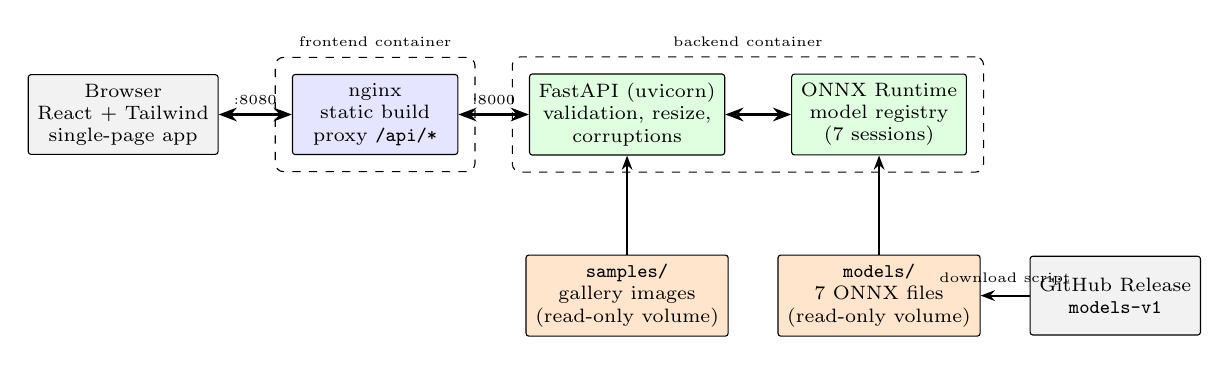
\begin{tikzpicture}[
    blk/.style={draw, rounded corners=1pt, minimum height=1.0cm, minimum width=2.1cm,
                align=center, font=\scriptsize},
    ext/.style={blk, fill=gray!10},
    fe/.style={blk, fill=blue!10},
    be/.style={blk, fill=green!12},
    st/.style={blk, fill=orange!20},
    box/.style={draw, dashed, rounded corners=3pt, inner sep=6pt},
    arr/.style={-{Stealth[length=1.8mm]}, thick},
    darr/.style={Stealth-Stealth, thick}
  ]
  \node[ext] (br)  at (0,0)    {Browser\\React + Tailwind\\single-page app};
  \node[fe]  (ng)  at (3.2,0)  {nginx\\static build\\proxy \texttt{/api/*}};
  \node[be]  (api) at (6.4,0)  {FastAPI (uvicorn)\\validation, resize,\\corruptions};
  \node[be]  (ort) at (9.6,0)  {ONNX Runtime\\model registry\\(7 sessions)};
  \node[st]  (mod) at (9.6,-2.3) {\texttt{models/}\\7 ONNX files\\(read-only volume)};
  \node[st]  (smp) at (6.4,-2.3) {\texttt{samples/}\\gallery images\\(read-only volume)};
  \node[ext] (rel) at (12.6,-2.3) {GitHub Release\\\texttt{models-v1}};

  \draw[darr] (br) -- node[above, font=\tiny] {:8080} (ng);
  \draw[darr] (ng) -- node[above, font=\tiny] {:8000} (api);
  \draw[darr] (api) -- (ort);
  \draw[arr] (mod) -- (ort);
  \draw[arr] (smp) -- (api);
  \draw[arr] (rel) -- node[above, font=\tiny] {download script} (mod);

  \node[box, fit=(ng), label={[font=\tiny]above:frontend container}] {};
  \node[box, fit=(api)(ort), label={[font=\tiny]above:backend container}] {};
\end{tikzpicture}%
}
.
\resizebox{\columnwidth}{!}{%
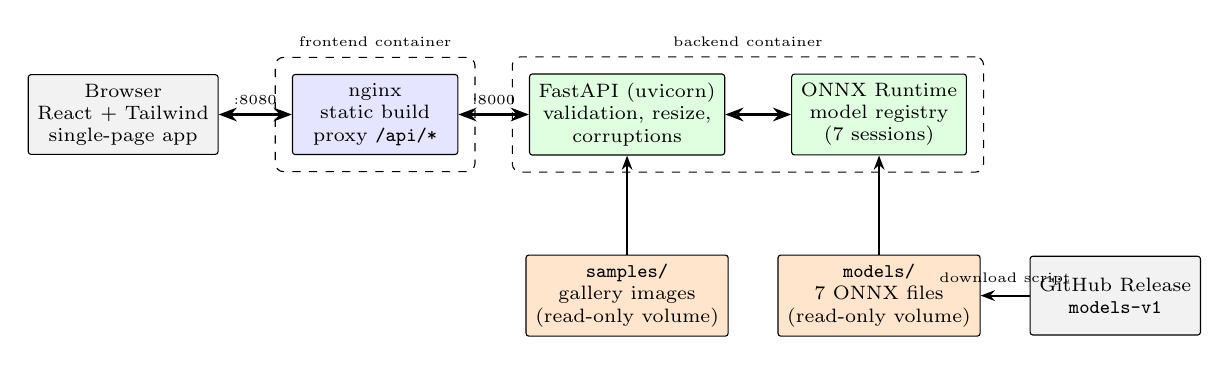
\begin{tikzpicture}[
    blk/.style={draw, rounded corners=1pt, minimum height=1.0cm, minimum width=2.1cm,
                align=center, font=\scriptsize},
    ext/.style={blk, fill=gray!10},
    fe/.style={blk, fill=blue!10},
    be/.style={blk, fill=green!12},
    st/.style={blk, fill=orange!20},
    box/.style={draw, dashed, rounded corners=3pt, inner sep=6pt},
    arr/.style={-{Stealth[length=1.8mm]}, thick},
    darr/.style={Stealth-Stealth, thick}
  ]
  \node[ext] (br)  at (0,0)    {Browser\\React + Tailwind\\single-page app};
  \node[fe]  (ng)  at (3.2,0)  {nginx\\static build\\proxy \texttt{/api/*}};
  \node[be]  (api) at (6.4,0)  {FastAPI (uvicorn)\\validation, resize,\\corruptions};
  \node[be]  (ort) at (9.6,0)  {ONNX Runtime\\model registry\\(7 sessions)};
  \node[st]  (mod) at (9.6,-2.3) {\texttt{models/}\\7 ONNX files\\(read-only volume)};
  \node[st]  (smp) at (6.4,-2.3) {\texttt{samples/}\\gallery images\\(read-only volume)};
  \node[ext] (rel) at (12.6,-2.3) {GitHub Release\\\texttt{models-v1}};

  \draw[darr] (br) -- node[above, font=\tiny] {:8080} (ng);
  \draw[darr] (ng) -- node[above, font=\tiny] {:8000} (api);
  \draw[darr] (api) -- (ort);
  \draw[arr] (mod) -- (ort);
  \draw[arr] (smp) -- (api);
  \draw[arr] (rel) -- node[above, font=\tiny] {download script} (mod);

  \node[box, fit=(ng), label={[font=\tiny]above:frontend container}] {};
  \node[box, fit=(api)(ort), label={[font=\tiny]above:backend container}] {};
\end{tikzpicture}%
}
.
\resizebox{\columnwidth}{!}{%
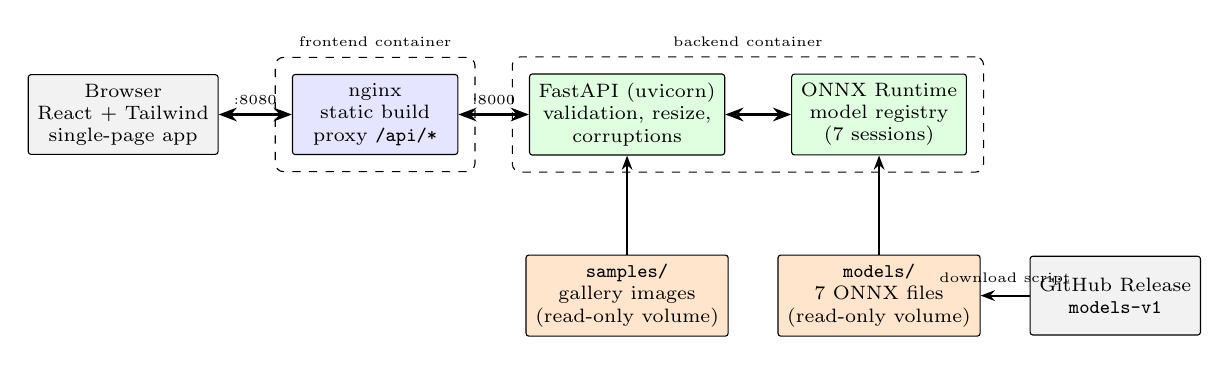
\begin{tikzpicture}[
    blk/.style={draw, rounded corners=1pt, minimum height=1.0cm, minimum width=2.1cm,
                align=center, font=\scriptsize},
    ext/.style={blk, fill=gray!10},
    fe/.style={blk, fill=blue!10},
    be/.style={blk, fill=green!12},
    st/.style={blk, fill=orange!20},
    box/.style={draw, dashed, rounded corners=3pt, inner sep=6pt},
    arr/.style={-{Stealth[length=1.8mm]}, thick},
    darr/.style={Stealth-Stealth, thick}
  ]
  \node[ext] (br)  at (0,0)    {Browser\\React + Tailwind\\single-page app};
  \node[fe]  (ng)  at (3.2,0)  {nginx\\static build\\proxy \texttt{/api/*}};
  \node[be]  (api) at (6.4,0)  {FastAPI (uvicorn)\\validation, resize,\\corruptions};
  \node[be]  (ort) at (9.6,0)  {ONNX Runtime\\model registry\\(7 sessions)};
  \node[st]  (mod) at (9.6,-2.3) {\texttt{models/}\\7 ONNX files\\(read-only volume)};
  \node[st]  (smp) at (6.4,-2.3) {\texttt{samples/}\\gallery images\\(read-only volume)};
  \node[ext] (rel) at (12.6,-2.3) {GitHub Release\\\texttt{models-v1}};

  \draw[darr] (br) -- node[above, font=\tiny] {:8080} (ng);
  \draw[darr] (ng) -- node[above, font=\tiny] {:8000} (api);
  \draw[darr] (api) -- (ort);
  \draw[arr] (mod) -- (ort);
  \draw[arr] (smp) -- (api);
  \draw[arr] (rel) -- node[above, font=\tiny] {download script} (mod);

  \node[box, fit=(ng), label={[font=\tiny]above:frontend container}] {};
  \node[box, fit=(api)(ort), label={[font=\tiny]above:backend container}] {};
\end{tikzpicture}%
}

\caption{Application architecture. Only the generator of Task~4 is deployed;
the discriminator is a training component.}
\label{fig:app_arch}
\end{figure}

\subsection{Backend}
The backend loads every ONNX model once at start-up. Uploads are checked
for type (PNG or JPEG) and size (at most 10\,MB); an upload or a gallery
sample is converted to RGB and resized directly to $128\times128$ (bicubic),
exactly as in training. Because the backend has no PyTorch, the three
corruptions are reimplemented with NumPy and OpenCV using the same
definitions and the fixed test severities; a test checks that the OpenCV blur
matches torchvision's within $3\times10^{-7}$. Hard routing runs the
classifier, applies the softmax and runs only the selected specialist, or
returns the input for a clean prediction; the soft mixture is a single ONNX
call that returns the image and the four weights. The reported inference
time is the time spent in the ONNX models. Invalid input returns HTTP 400 or
413 with a message, and a missing model returns 503. Table~\ref{tab:api}
lists the endpoints.

\begin{table}[t]
\centering
\caption{Backend API (all paths under \texttt{/api}).}
\label{tab:api}
\scriptsize
\begin{tabular}{@{}lp{0.45\columnwidth}@{}}
\toprule
Endpoint & Purpose / response \\
\midrule
\texttt{GET /health} & status, loaded models, last inference time \\
\texttt{GET /samples}, \texttt{/samples/\{id\}} & gallery images \\
\texttt{POST /restore/universal} & Task 1: input, output, corruption settings, time \\
\texttt{POST /restore/hard-routing} & Task 2: + four probabilities, predicted class, selected expert \\
\texttt{POST /restore/soft-moe} & Task 3: + four routing weights, top branch \\
\texttt{POST /sketch} & Task 4: photo and sketch for style 1, 2 or 3 \\
\bottomrule
\end{tabular}
\\[3pt]
\parbox{\columnwidth}{\footnotesize Restore requests take a file or a
sample id, a corruption (\texttt{none}, \texttt{salt\_pepper},
\texttt{blur}, \texttt{occlusion}), a severity (low, medium, high) and an
optional seed.}
\end{table}

\subsection{Frontend}
The frontend is written in React with Tailwind CSS. A sidebar gives access
to an overview page and the four workspaces---\emph{Universal Restoration},
\emph{Hard-Routed Restoration}, \emph{Soft Mixture-of-Experts Restoration}
and \emph{Face-to-Sketch Generator}---and shows a system-status card that
polls the health endpoint every 10\,s. The restoration workspaces accept an
upload (including an already corrupted image) or a gallery sample, let the
user choose a corruption and severity, and show the input, the restored
output, the corruption settings and the inference time; the hard-routing
workspace adds the four class probabilities, the predicted corruption and
the selected expert, and the mixture workspace shows the four routing
weights with the strongest contributors highlighted. The sketch workspace
accepts an upload or a webcam capture, offers Styles 1--3, shows photo and
sketch side by side and lets the user download the result.
Fig.~\ref{fig:app_screens} shows the running application.

\begin{figure*}[t]
\centering
\begin{minipage}{0.49\textwidth}\centering
\figOrTodo{figures/app_universal.png}{\linewidth}{Screenshot: Universal Restoration with a corrupted sample}
\end{minipage}\hfill
\begin{minipage}{0.49\textwidth}\centering
\figOrTodo{figures/app_hard_routed.png}{\linewidth}{Screenshot: Hard-Routed Restoration with probabilities and selected expert}
\end{minipage}\\[6pt]
\begin{minipage}{0.49\textwidth}\centering
\figOrTodo{figures/app_soft_moe.png}{\linewidth}{Screenshot: Soft Mixture-of-Experts Restoration with routing weights}
\end{minipage}\hfill
\begin{minipage}{0.49\textwidth}\centering
\figOrTodo{figures/app_face_to_sketch.png}{\linewidth}{Screenshot: Face-to-Sketch Generator with photo and sketch side by side}
\end{minipage}
\caption{The running application with the trained models: (top left)
Universal Restoration, (top right) Hard-Routed Restoration, (bottom left)
Soft Mixture-of-Experts Restoration, (bottom right) Face-to-Sketch Generator.}
\label{fig:app_screens}
\end{figure*}

\subsection{Model distribution}
Model files are not committed. The seven ONNX files are attached to a
GitHub Release (\texttt{models-v1}) and fetched by a standard-library Python
script or by hand into \file{models/}. Git LFS was considered, but its free
tier provides 1\,GB of storage and 1\,GB of download bandwidth per month,
and the Task~4 generator alone is about 168\,MB at 64 base channels, so a
few clones could exhaust the quota; release assets have no comparable
bandwidth quota.
% TODO: create the models-v1 release once the trained models exist, and update the generator size to the trained configuration.
\TODO{Create the \texttt{models-v1} release; update the file sizes to the
trained configurations.}

% =====================================================================
\section{Limitations}
\label{sec:limitations}

\begin{itemize}
  \item \emph{Single runs.} Each configuration is trained once with seed 42;
  we report no variance across seeds, so small differences between systems
  should be read with caution.
  \item \emph{Short Optuna trials.} Trials use 8--25 epochs, far fewer than
  the final schedules; the ranking of configurations after a short run may
  differ from their ranking after full training.
  \item \emph{Fixed validation weighting.} The objective $J$ uses the
  weights 0.8/0.2, which may slightly favour trials whose training $\alpha$
  or $\lambda_1$ is close to 0.8.
  \item \emph{Occlusion is ill-posed.} Content hidden by a black rectangle is
  not present in the input; any reconstruction of it is an inference from the
  surrounding context, not a recovery.
  \item \emph{GAN selection criterion.} Selecting Task~4 models by paired
  L1/SSIM rewards correct structure but may favour smoother sketches over
  sharper but slightly misaligned strokes; FID was not used because of the
  small validation set.
  \item \emph{Gate criteria.} The thresholds for inactive and dominating
  experts are judgement calls.
  \item \emph{Preprocessing.} Direct resizing distorts the aspect ratio of
  non-square images, and $128\times128$ limits the detail that any of the
  models can restore or draw.
  \item \emph{Application corruptions.} The application offers only the three
  fixed test severities per corruption, not the continuous training ranges.
  \item \emph{Literature.} Several design arguments rely on sources that must
  still be read first-hand.
  % TODO: remove this item once every cited work has been read.
\end{itemize}
% TODO(results): add limitations revealed by the results (e.g. failure modes that no system handles).
\TODO{Add limitations revealed by the results.}

% =====================================================================
\section{Conclusion}
\label{sec:conclusion}

We built four generative image systems on a shared, checkable data
pipeline: a universal denoising autoencoder with an explicit spatial
bottleneck, a hard-routing system with an exactly balanced classifier and
three specialists, a soft mixture-of-experts that starts from those trained
components and is guarded against routing collapse, and a style-conditioned
pix2pix-style GAN for face-to-sketch generation. All four are tuned with
Optuna, tracked in W\&B, verified after ONNX export and available in one
containerised web application.
% TODO(results): conclusions from the results.
\TODO{State the main findings: which restoration approach worked best on
which corruption, what the gate learned, how well the style condition was
used, and what we would change next.}

\section*{Code and Demonstration}
Source code, configuration files, Optuna studies, manifests and execution
instructions:
\url{https://github.com/aleenababar04/genai-assignment-1}.\\
Demonstration video:
% TODO: insert the YouTube link (link only).
\TODO{YouTube link}.

% =====================================================================
\bibliographystyle{IEEEtran}
\bibliography{references}

% =====================================================================
\appendices

\section{Use of AI Tools}
\label{app:ai}

AI tools were used for research, coding, interface design, debugging and
documentation. The student remains responsible for every component. The
list below reproduces the AI-use log kept during the work
(\file{docs/ai_use_log.md}); for each use it states what the tool was used
for and how its output was verified or corrected. Items marked
\TODO{\dots} are verification steps that have not yet been completed.

\begin{enumerate}
\item \textbf{2026-10-02, Claude Code (Claude Opus).}
\emph{Used for:} reading the assignment brief and producing the eight-phase plan.
\emph{Verification:} the plan was produced from the brief's PDF.
% TODO: Pending item from docs/ai_use_log.md.
\TODO{Pending: own check of the plan against the brief, section by section.}

\item \textbf{2026-10-02, Claude Code (Claude Opus), with two subagents.}
\emph{Used for:} scaffolding the repository: folder layout,
\file{.gitignore}, requirements files, \file{src/utils} (seed, config,
tracking), \file{configs/base.yaml}, tests, log templates, README skeleton,
Kaggle launcher notes.
\emph{Verification:} \texttt{pytest} in the local virtual environment: 4
passed (seeding reproducibility, config round trip, Optuna storage path,
study reload). Two errors in the generated files were found and corrected:
\file{manifests_dir} pointed at the git-ignored \file{data/manifests}
(changed to \file{manifests}), and the \file{.gitignore} rule \file{data/}
also ignored \file{src/data/} (changed to \file{/data/}).
% TODO: Pending item from docs/ai_use_log.md.
\TODO{Pending: own line-by-line read of \file{src/utils}.}

\item \textbf{2026-10-02, Claude Code (Claude Opus).}
\emph{Used for:} diagnosing the Smart App Control import errors and fixing
the local environment.
\emph{Verification:} the tool's prediction that a Windows Security exclusion
would have no effect was wrong for \texttt{onnx} and \texttt{scikit-learn}:
after adding the exclusion both imported. SQLAlchemy stayed blocked; the tool
reinstalled it without compiled extensions, checked by re-running
\texttt{pytest} (3 passed, 1 failed before; 4 passed after).

\item \textbf{2026-10-02, Claude Code (Claude Opus).}
\emph{Used for:} filling in the entries of the decision log and the AI-use
log (ongoing).
\emph{Verification:} entries record only what was actually run or observed in
the session; documentation not yet read first-hand is marked as such in the
decision log.

\item \textbf{2026-10-03, Claude Code (Claude Opus), with two subagents.}
\emph{Used for:} Phase~1 data pipeline (\file{src/data/corruptions.py},
\file{prepare_pet.py}, \file{manifests.py}, \file{pet_dataset.py},
\file{src/evaluation/preview_corruptions.py}) and their tests.
\emph{Verification:} full test suite run locally: 47 passed (25 corruption,
11 preparation, 7 manifest/dataset, 4 utility tests). The occlusion sampler's
retry rate was measured over 2,000 draws. The pipeline was then run on the
real dataset: image and manifest counts matched the expected values,
occlusion coverage was measured per severity and the preview grid was
inspected. That run exposed blurred values slightly above 1.0, fixed by
clamping to $[0,1]$.
% TODO: Pending item from docs/ai_use_log.md.
\TODO{Pending: own read-through of the four data modules.}

\item \textbf{2026-10-03, Claude Code (Claude Opus), with one subagent.}
\emph{Used for:} drafting the Google Stitch prompt pack
(\file{docs/stitch_prompts.md}).
\emph{Verification:} the prompts were not tried in Stitch by the tool.
% TODO: Pending item from docs/ai_use_log.md.
\TODO{Pending: note which prompts were used, what Stitch produced and what was changed.}

\item \textbf{2026-10-03, Claude Code (Claude Opus), with two subagents.}
\emph{Used for:} Phase~2 code for Task~1 (\file{src/models/autoencoder.py},
\file{src/training/losses.py}, \file{train_udae.py},
\file{src/evaluation/metrics.py}, \file{figures.py}, \file{eval_udae.py},
\file{src/export/export_onnx.py}, \file{configs/task1_udae.yaml}, the Kaggle
notebook and tests).
\emph{Verification:} test suite: 82 passed. A tiny CPU run exercised every
script end to end (Optuna with 2 trials, final training, evaluation on 20 test
images, ONNX export with maximum PyTorch--ONNX difference $5.96\times10^{-8}$);
these were plumbing checks on an untrained model, not results. A short CPU
training run (30 batches per epoch) confirmed that the validation objective
falls (0.320 before, 0.282 after one epoch).
% TODO: Pending item from docs/ai_use_log.md.
\TODO{Pending: the real Kaggle run and own read-through of the model and training script.}

\item \textbf{2026-10-03, Claude Code (Claude Opus), with three subagents.}
\emph{Used for:} Phase~3 code for Task~2 (\file{src/models/classifier.py},
\file{src/data/balanced.py}, \file{src/models/hard_router.py},
\file{src/evaluation/classification.py}, \file{eval_task2.py},
\file{src/training/train_classifier.py}, \file{train_specialists.py}, the two
Task~2 configs, the Task~2 export and Kaggle notebook).
\emph{Verification:} test suite: 121 passed (new: 17 classifier/balanced-batch
tests, 8 classification-metric tests, 14 routing tests). Each subagent's
module was tested on its own, then every Task~2 script was run end to end on
CPU with a few batches (both Optuna searches, both final trainings,
evaluation on 5 test images, ONNX export of the four models with maximum
PyTorch--ONNX difference at most $5.96\times10^{-8}$); these were plumbing
checks on untrained models and their outputs were deleted. The smoke run
showed that clean images returned unchanged score the capped 100\,dB PSNR and
inflate overall averages, so a ``corrupted/all'' summary row and an SSIM-loss
column for misrouted images were added (122 tests passed afterwards).
% TODO: Pending item from docs/ai_use_log.md.
\TODO{Pending: the real Kaggle run and own read-through.}

\item \textbf{2026-10-03, Claude Code (Claude Opus), with two subagents.}
\emph{Used for:} Task~3 code (\file{src/models/soft_moe.py},
\file{src/evaluation/routing_analysis.py}, \file{src/training/train_moe.py},
\file{src/evaluation/eval_moe.py}, the Task~3 export, config and Kaggle
notebook).
\emph{Verification:} new tests: 18 for the mixture (mixing equals the
hand-computed weighted sum, frozen experts get no gradients and keep
batch-normalisation statistics, full-pipeline ONNX matches PyTorch) and 10
for the gate analysis. A CPU smoke run (with throwaway Task~2 models)
exercised the Optuna search, final training, test evaluation with gate
analysis and the single-graph ONNX export (maximum PyTorch--ONNX difference
$1.19\times10^{-7}$ on the image, $2.98\times10^{-8}$ on the weights); its
outputs were deleted. The first attempt hit the one-hour background limit on
the shared CPU and the remaining steps were rerun. While it ran, validation
was found to pass over the data twice; it was changed to collect the routing
weights in the same pass.
% TODO: Pending item from docs/ai_use_log.md.
\TODO{Pending: the real Kaggle run and own read-through.}

\item \textbf{2026-10-03, Claude Code (Claude Opus), with two subagents.}
\emph{Used for:} Task~4 code (\file{src/models/cgan.py},
\file{src/data/prepare_fs2k.py}, \file{src/data/fs2k_dataset.py},
\file{src/training/train_cgan.py}, \file{src/evaluation/eval_cgan.py}, the
Task~4 export, config and Kaggle notebook). The FS2K folder layout and
photo-to-sketch naming rule were looked up by the tool on the FS2K GitHub page.
\emph{Verification:} new tests: 16 for the networks (style changes $G$ and $D$
outputs, gradients reach both embeddings, ONNX matches within $10^{-4}$ for all
three styles) and 17 for the data (stratified split, identical augmentation of
photo and sketch, on a synthetic FS2K tree). An end-to-end CPU smoke run on a
tiny fake cache covered the Optuna trial, final training, evaluation and ONNX
export (maximum difference $5.96\times10^{-8}$); its outputs were deleted.
% TODO: Pending item from docs/ai_use_log.md.
\TODO{Pending: confirm the FS2K layout against the real download.}

\item \textbf{2026-10-03, Claude Code (Claude Opus), with one subagent.}
\emph{Used for:} the FastAPI backend (image validation and preprocessing,
NumPy/OpenCV corruptions for the application, ONNX model registry, the five
required operations plus health and samples endpoints, Dockerfile, tests) and
the choice of six test-set pet images as application samples.
\emph{Verification:} 73 backend tests passed after installing the backend
packages, including a check that the OpenCV blur matches torchvision's within
$3\times10^{-7}$ and that upload validation rejects non-images and oversized
files. The server was started locally and the health endpoint correctly listed
all seven models as not loaded.

\item \textbf{2026-10-03, Claude Code (Claude Opus), with one subagent.}
\emph{Used for:} the React + Tailwind frontend, \file{docker-compose.yml}, the
nginx proxy configuration, README run instructions and
\file{scripts/download_models.py}.
\emph{Verification:} \texttt{npm run build} succeeded; the development server
was checked against the real backend (health, samples, 503 and 400 error
cards) and the pages were exercised in headless Chrome by the subagent.
\texttt{docker compose up --build} built both images and started them: the
backend became healthy, \texttt{http://localhost:8080} served the application
(including client-side routes), and the health, samples, sample-image and
restore requests (503 ``model not loaded'', as expected without models) all
worked through the nginx proxy.
% TODO: Pending item from docs/ai_use_log.md.
\TODO{Pending: the visual comparison with the Stitch design, and a run with the real models.}

\item \textbf{2026-10-03, Claude Code (Claude Opus), with one subagent.}
\emph{Used for:} drafting this report's LaTeX source (structure, methodology
text from the decision log and the code, TikZ diagrams, empty result tables)
and looking up the bibliographic details of the cited works on Crossref,
arXiv, the NeurIPS proceedings pages, Distill and the FS2K repository.
\emph{Verification:}
% TODO: add this row to docs/ai_use_log.md as well; record how the draft was checked.
\TODO{Not yet verified: compile on Overleaf, check every methodological
statement against the code and the decision log, read every cited work
first-hand, and record the corrections made here and in
\file{docs/ai_use_log.md}.}
\end{enumerate}

\end{document}
